\documentclass[12pt, a4paper]{report}

% --- PAQUETES ESENCIALES ---
\usepackage[utf8]{inputenc}
\usepackage[T1]{fontenc}
\usepackage[spanish, es-tabla]{babel} % Idioma español y renombra "Cuadro" a "Tabla"

% --- MATEMÁTICAS ---
\usepackage{amsmath}
\usepackage{amsfonts}
\usepackage{amssymb}

% --- GRÁFICOS Y DISEÑO ---
\usepackage{xcolor}
\usepackage{graphicx}
\usepackage{tikz}
\usetikzlibrary{arrows.meta, positioning}
\usetikzlibrary{babel} % evita el choque entre los caracteres activos de babel-spanish y TikZ/pgf
\usepackage{pgfplots}
\pgfplotsset{compat=1.18}

% --- Colores para los esquemas de agregación circular (Figura TSP3) ---
\definecolor{cfwd}{RGB}{20,80,160}   % avance en el sentido de rotación
\definecolor{cbwd}{RGB}{175,35,35}   % retroceso (penalizado)
% --- Colores del esquema de la arquitectura modular (Figura 2.2) ---
\definecolor{cprm}{RGB}{200,110,20}  % parámetros configurables
\definecolor{cpar}{RGB}{20,120,110}  % mejora: eficiencia computacional
\definecolor{creg}{RGB}{120,55,150}  % mejora: regularización FMM
\definecolor{cagg}{RGB}{30,115,60}   % mejora: orden representativo
\newcommand{\bnditem}[2]{\textcolor{#1}{\textbullet}\ #2}
\newcommand{\cf}[1]{\textcolor{cfwd}{#1}}
\newcommand{\cb}[1]{\textcolor{cbwd}{#1}}
\usepackage[margin=2.5cm]{geometry}
\usepackage{setspace}
\onehalfspacing % Interlineado 1.5, obligatorio/estándar. ¡Sin errores de grupo!

% --- CITAS ---
\usepackage[numbers]{natbib}

% --- LISTAS ---
\usepackage{enumitem}

% --- ENLACES Y METADATOS ---
\usepackage[hidelinks]{hyperref}
\usepackage[nottoc]{tocbibind} % ¡Esta es la línea mágica!
\begin{document}


\begin{titlepage}
    \centering

    \includegraphics[width=0.4\textwidth]{./images/logo-cuatricromia.pdf}\par\vspace{1cm}

    {\scshape\LARGE Universidad de Valladolid \par}
    \vspace{0.5cm}
    {\scshape\Large Facultad de Ciencias\par}
    \vspace{2cm}

    {\huge\bfseries Extensión y optimización del procedimiento CIRCUST de reconstrucción temporal\par}
    \vspace{1.5cm}

    {\Large \textit{Trabajo de Fin de Grado en Estadística}\par}
    \vspace{2cm}

    \begin{minipage}[t]{0.4\textwidth}
        \begin{flushleft} \large
            \emph{Autor:}\\
            \textbf{Samuel Ortega Bustos}
        \end{flushleft}
    \end{minipage}
    ~
    \begin{minipage}[t]{0.5\textwidth}
        \begin{flushright} \large
            \emph{Tutores:} \\
            \textbf{Yolanda Larriba González} \\
            \textbf{Juan Camilo Yepes Borrero}
        \end{flushright}
    \end{minipage}\\[2cm]

    \vfill

    {\large \textbf{Curso Académico 2025-2026} \par}
    \vspace{0.5cm}
    {\large \today \par}
\end{titlepage}

% ==========================================
% RESUMEN / ABSTRACT
% ==========================================
\pagenumbering{roman} % Números romanos para los índices

\begin{abstract}
La estimación de la fase circadiana a partir de datos transcriptómicos representa un reto central en cronobiología, especialmente en estudios humanos donde las etiquetas temporales suelen ser inaccesibles por restricciones éticas o clínicas. El algoritmo CIRCUST, basado en el Análisis de Componentes Principales Circulares (CPCA), ha demostrado ser una herramienta prometedora para la reconstrucción del orden temporal. Sin embargo, su implementación actual carece de la modularidad necesaria y de mecanismos para ajustar covariables o manejar muestreos dispersos.

Este trabajo presenta una re-implementación modular y eficiente de CIRCUST en Python, junto con un refinamiento metodológico profundo. Las mejoras incluyen la integración de ajustes por covariables y una optimización de la ordenación circular para mejorar la inferencia de fase. Además, se ha desarrollado un marco de simulación para evaluar sistemáticamente la robustez del modelo frente a perturbaciones como el ruido y los efectos por lotes. Finalmente, el pipeline mejorado se valida utilizando conjuntos de datos transcriptómicos reales del cerebro humano post-mortem, demostrando una mayor precisión y relevancia biológica.

\textbf{Palabras clave:} Cronobiología, Transcriptómica, Ordenación Circular, CPCA, Python.
\end{abstract}

\renewcommand{\abstractname}{Abstract}
\begin{abstract}
Estimating circadian phase from transcriptomic data is a central challenge in chronobiology, particularly in human studies where time-of-day labels are often unavailable. The CIRCUST algorithm, based on Circular Principal Component Analysis (CPCA), offers a promising approach for temporal order reconstruction. However, its current implementation lacks modularity, extensibility, and built-in mechanisms to adjust for covariates or to handle sparse sampling patterns.

This project presents a modular and efficient re-implementation of CIRCUST in Python, alongside a deep methodological refinement. Improvements include the integration of covariate adjustments and enhanced circular ordering for better phase inference. Furthermore, a simulation framework is developed to systematically evaluate robustness against perturbations such as noise and batch effects. Finally, the improved pipeline is validated using real post-mortem human brain transcriptomic datasets, demonstrating improved accuracy and biological relevance.

\textbf{Keywords:} Chronobiology, Transcriptomics, Circular Ordering, CPCA, Python.
\end{abstract}

% ==========================================
% ÍNDICES
% ==========================================
\tableofcontents
\newpage
\listoffigures
\newpage
\listoftables
\newpage

% ==========================================
% CUERPO DEL TRABAJO
% ==========================================
\pagenumbering{arabic}

\chapter{Introducción}

\section{El sistema circadiano: ritmos, reloj molecular y genes circadianos}
Los ritmos circadianos subyacen a una gran variedad de procesos biológicos en prácticamente todos los organismos vivos, desde cianobacterias hasta seres humanos \cite{bell-pedersen2005}. Estos ritmos se manifiestan en distintos niveles de organización biológica, incluyendo procesos fisiológicos, hormonales y moleculares, como la regulación de la temperatura corporal, el ritmo cardíaco, la secreción de cortisol y melatonina o la expresión génica. Sincronizados principalmente por el ciclo diario de luz y oscuridad, los ritmos circadianos desempeñan un papel fundamental en la regulación y coordinación temporal de procesos fisiológicos, metabólicos y conductuales a lo largo de las 24 horas del día \cite{takahashi2017, halberg1969, mohawk2012, mure2018}.

En mamíferos, la organización del sistema circadiano es jerárquica \cite{gomezabellan2012}: un oscilador central, conocido como reloj circadiano central y localizado en el núcleo supraquiasmático del hipotálamo \cite{klein1991}, recibe información lumínica desde la retina y la utiliza para sincronizarse con el ciclo externo de luz y oscuridad. Este reloj actúa como marcapasos y coordina osciladores periféricos presentes en órganos y tejidos. La correcta sincronización entre estos relojes resulta esencial para mantener la coordinación temporal de los procesos fisiológicos y metabólicos del organismo, así como su adecuada adaptación a las condiciones ambientales. A nivel molecular, tanto el reloj central como los relojes periféricos se sustentan en redes de genes reloj organizadas en bucles de retroalimentación entre la transcripción y la traducción, que generan oscilaciones de expresión génica con un periodo cercano a las 24 horas y permiten mantener la ritmicidad circadiana en cada tejido \cite{takahashi2017, ueda2005}. La Figura~\ref{fig:jerarquia} muestra una esquematización de dicha estructura jerárquica.

\begin{figure}[htbp]
\centering
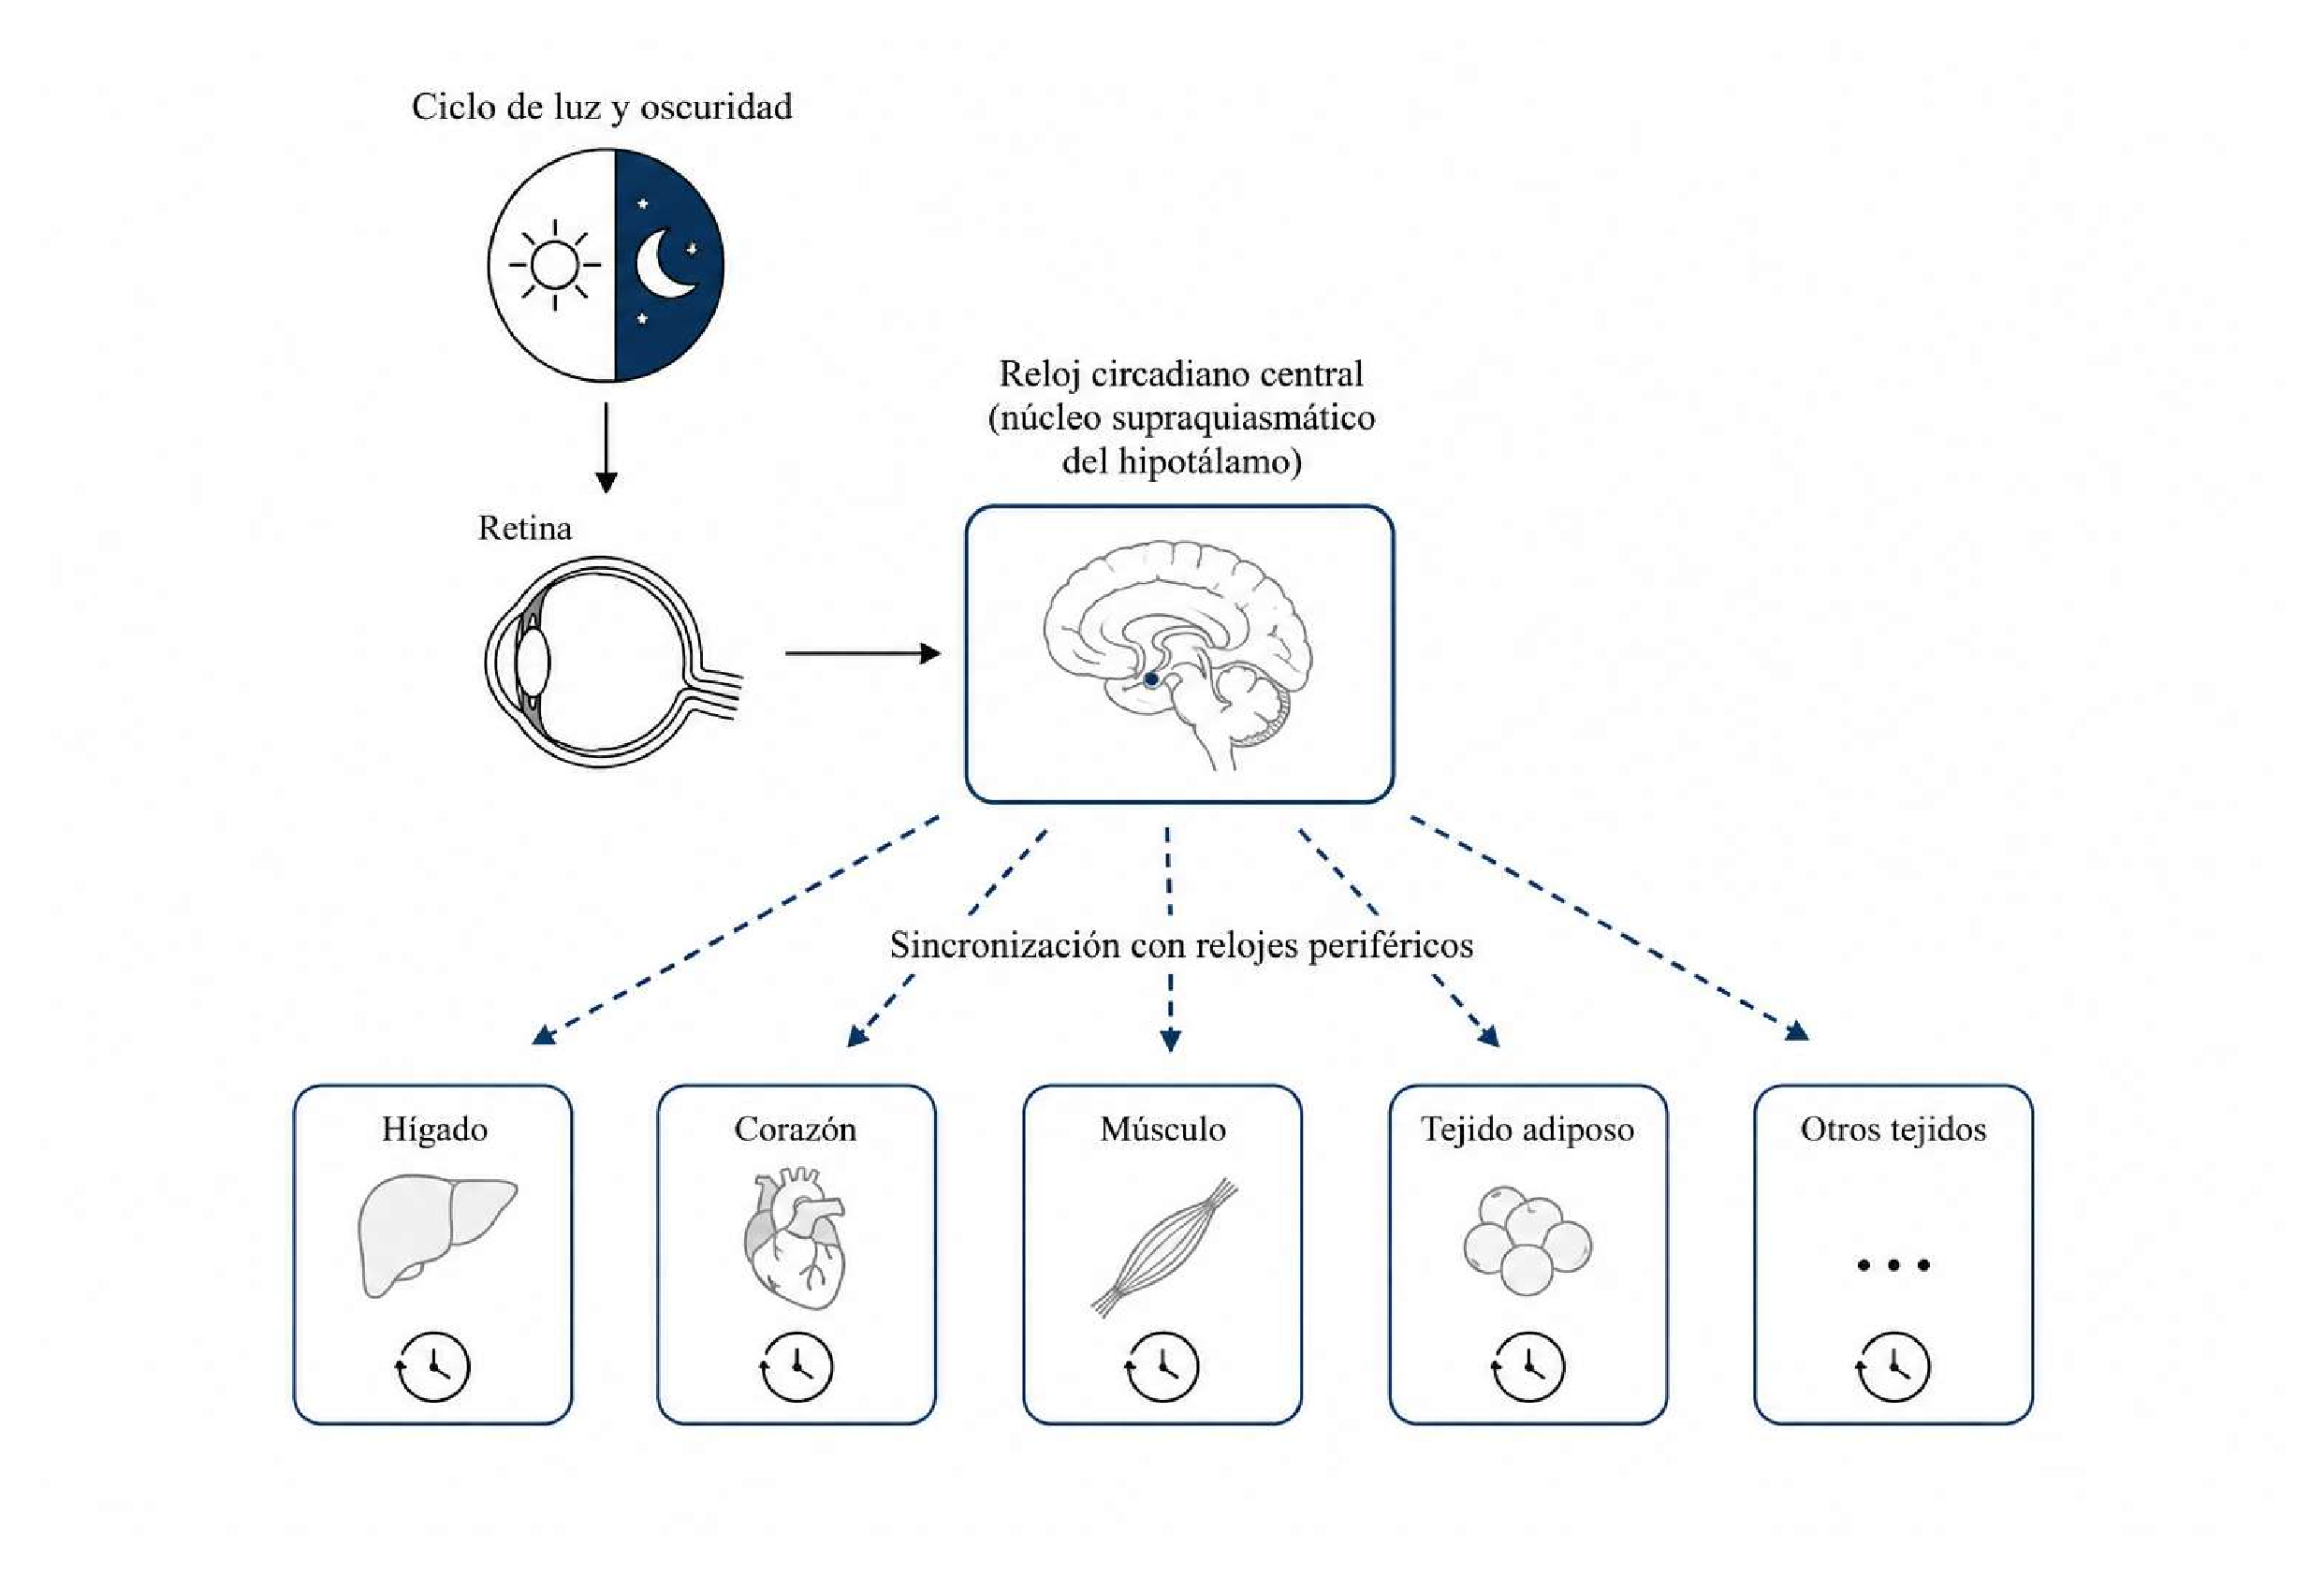
\includegraphics[width=0.85\textwidth]{images/imagenEsquematica.pdf}
\caption[Organización jerárquica del sistema circadiano.]{Esquematización de la organización jerárquica del sistema circadiano: el reloj central se sincroniza con la luz a través de la retina, así como con los relojes periféricos de los distintos órganos o tejidos.}
\label{fig:jerarquia}
\end{figure}

Esta arquitectura jerárquica da lugar a patrones de expresión génica rítmica específicos de cada tejido. Denominaremos genes circadianos a aquellos cuya expresión presenta oscilaciones con un periodo aproximado de 24 horas, véase Figura~\ref{fig:oscilacion}. Estos genes desempeñan un papel fundamental en la regulación temporal de procesos celulares y fisiológicos, favoreciendo que las distintas funciones biológicas se ejecuten de forma coordinada a lo largo del día. En particular, el instante de máxima expresión génica (pico de expresión) se encuentra estrechamente relacionado con el momento del día en que el gen ejerce su función biológica \cite{ruan2021, bahammam2023}.


\begin{figure}[htbp]
\centering
\pgfmathsetseed{42}
\begin{tikzpicture}
\begin{axis}[
    width=0.85\textwidth, height=5cm,
    xlabel={Hora del día}, ylabel={Nivel de expresión},
    xmin=0, xmax=24, ymin=-1.6, ymax=2.0,
    xtick={0,6,12,18,24},
    ytick=\empty,
    axis lines=left,
    clip=false,
]
\addplot[only marks, mark=*, mark size=1.1pt, gray!70, domain=0:24, samples=44]
    {cos(360*(x-12.8)/24) + 0.15*cos(2*360*(x-12.8)/24) + 0.30*sin(2*360*(x-12.8)/24) + 0.20*rand};

\addplot[thick, blue, domain=0:24, samples=200]
    {cos(360*(x-12.8)/24) + 0.15*cos(2*360*(x-12.8)/24) + 0.30*sin(2*360*(x-12.8)/24)};
\draw[dashed, gray] (axis cs:14,-1.6) -- (axis cs:14,1.32);
\node at (axis cs:14,1.32) [above, yshift=2pt, font=\small] {Pico (máxima expresión)};
\end{axis}
\end{tikzpicture}
\caption[Esquematización del ritmo circadiano subyacente en datos de expresión de un gen circadiano en 24 horas.]{Esquematización del ritmo circadiano subyacente en datos de expresión de un gen circadiano en 24 horas. Los puntos representan las observaciones de expresión y la línea azul el patrón oscilatorio subyacente. El pico marca el instante de máxima expresión y se relaciona con el momento del día en que el gen realiza su función biológica.}
\label{fig:oscilacion}
\end{figure}


En el contexto de la biología circadiana humana, ámbito en el que se centra este trabajo, la relevancia de los ritmos y genes circadianos ha sido ampliamente documentada, existiendo evidencia de variaciones temporales en resultados clínicos y en la respuesta a distintas intervenciones terapéuticas, como la cirugía cardíaca, la quimioterapia o la respuesta inmune \cite{fudulu2021, marcu2024, ince2023}. En contraposición, se ha evidenciado que la desalineación crónica del reloj circadiano, asociada al trabajo por turnos (\textit{shift work}), al \textit{jet lag} social o a la exposición nocturna a luz artificial, constituye un factor de riesgo para trastornos metabólicos, enfermedades cardiovasculares, trastornos neurodegenerativos y diversos tipos de cáncer \cite{sulli2018, sahar2009}.

\section{Análisis de genes circadianos humanos: modelos para el análisis de señales oscilatorias}

La identificación y caracterización de los genes circadianos constituye un reto fundamental en biología circadiana, ya que permite comprender cómo se organizan y sincronizan los procesos moleculares y fisiológicos con los ciclos ambientales, sentando las bases para el desarrollo de estrategias de cronomedicina y medicina de precisión.

Los modelos para el análisis de señales oscilatorias más empleados en cronobiología para describir e identificar ritmos circadianos son los modelos armónicos sinusoidales, normalmente con un único componente de periodo fijado, por ejemplo 24 horas, entre los que destaca el modelo Cosinor \cite{cosinor}. Este enfoque representa la señal mediante una función cosenoidal, habitualmente con un periodo prefijado, y permite estimar parámetros interpretables como la amplitud, la fase y el nivel medio de expresión. Este tipo de aproximación resulta útil por su sencillez e interpretabilidad, pero puede ser limitada cuando las señales presentan formas asimétricas o patrones de oscilación más complejos.

Como alternativa, existen métodos no paramétricos como RAIN \cite{rain2014} o JTK\_CYCLE \cite{jtkcycle2010} o más recientemente ORI \cite{larriba2020}, que permiten identificar patrones rítmicos sin imponer una forma funcional tan rígida. Sin embargo, no siempre proporcionan parámetros directamente interpretables desde el punto de vista biológico, lo que puede dificultar la caracterización posterior de las diferencias entre grupos o regiones.

En este contexto, destacan los modelos FMM (Frequency Modulated Möbius) \cite{fmmAlgorithm}, una familia de modelos paramétricos flexibles diseñada para modelizar señales oscilatorias complejas mediante un conjunto reducido de parámetros con interpretación fisiológica. Estos modelos constituyen una alternativa especialmente adecuada para describir patrones de expresión génica no sinusoidales o asimétricos. Además, su sólido fundamento matemático ha favorecido el desarrollo de numerosas extensiones metodológicas y su aplicación  al análisis de señales oscilatorias en distintos ámbitos de la cronobiología.


La aplicación de estos modelos resulta especialmente relevante en el estudio de la expresión génica circadiana. En este ámbito, la identificación y caracterización precisa de los genes circadianos, así como de sus relaciones intra- e intertisulares, constituye uno de los principales retos de la cronobiología, ya que es fundamental para comprender la regulación y coordinación de los relojes circadianos entre tejidos humanos y su interacción con el entorno. 

Este objetivo se materializa en los denominados atlas de expresión circadiana, que describen la regulación temporal de la expresión génica a escala del organismo y constituyen un recurso clave para el descubrimiento de biomarcadores temporales y el desarrollo de estrategias terapéuticas \textit{time-aware} \cite{zhang2014, dyar2018, mure2018, ruben2018, wei2022, larriba2023}. Hasta la fecha se dispone de atlas de expresiones circadianas humanas para un número muy reducido de tejidos, generalmente periféricos. Esta limitación ha llevado tradicionalmente a recurrir tradicionalmente a estudios en especies homólogas, como ratones o babuinos, donde es posible obtener muestras in vivo. Aunque estos modelos han servido como referencia para guiar la toma de decisiones en humanos, es evidente que pueden introducir sesgos relevantes.

\section{Atlas de expresiones circadianas humanas. El problema de estimación del orden temporal}

Para abordar el problema de la identificación y caracterización de genes circadianos humanos orientado al avance en la construcción de atlas de expresión génica circadiana en humanos, así como al estudio de la interrelación entre tejidos de estos genes, resulta imprescindible disponer de matrices de datos de expresión génica humana a lo largo de las 24 horas en una amplia colección de tejidos y órganos. Sin embargo, la obtención de dichos datos transcriptómicos longitudinales no es viable por razones clínicas y éticas, lo que motiva el uso de datos de expresión \textit{post mortem} en estudios transcriptómicos humanos.

\subsubsection{Limitaciones de los datos de expresión génica humana}

A diferencia de lo que ocurre en estudios experimentales con modelos animales, donde la variable temporal puede observarse de forma controlada mediante muestreos realizados a distintas horas del día, en humanos este tipo de diseño no es viable debido al riesgo que implica la obtención de biopsias seriadas de tejidos internos a lo largo del día. Como consecuencia, el análisis transcriptómico en humanos habitualmente se realiza a partir de estudios transversales con muestras \textit{post mortem}, en las que el tiempo biológico interno de cada individuo no se observa directamente y debe ser inferido a partir de la información disponible.

Como aproximación a esta limitación, algunos estudios utilizan la hora de muerte (\textit{TOD}, del inglés \textit{Time of Death}) como referencia temporal. Sin embargo, emplear directamente esta variable puede inducir una ordenación inadecuada de las muestras, ya que la hora de fallecimiento no tiene por qué coincidir con la fase circadiana real del individuo. Factores como el cronotipo, los hábitos de sueño, determinadas patologías, la medicación o las condiciones previas al fallecimiento pueden provocar discrepancias entre el tiempo externo registrado y el estado circadiano interno.

A esta incertidumbre temporal se añade la elevada variabilidad característica de los estudios transcriptómicos humanos. Por un lado, existe variabilidad técnica derivada de la degradación del ARN (Ácido ribonucleico), de errores sistemáticos o aleatorios en los dispositivos de medición y de la heterogeneidad de los protocolos experimentales entre laboratorios. Por otro, al tratarse de datos transversales procedentes de individuos distintos, también existe una importante variabilidad biológica y clínica. Variables como la edad, el sexo, la causa de la muerte, el estado clínico o la historia individual de sueño pueden influir en la expresión génica y dificultar la separación entre la variabilidad interindividual y la asociada al momento circadiano.

Además, los estudios transcriptómicos humanos \textit{post mortem} suelen presentar una cobertura temporal irregular a lo largo del ciclo circadiano, ya que determinadas franjas horarias se encuentran sobrerrepresentadas mientras que otras apenas disponen de muestras \cite{kimura2023, gorczyca2025}. Esta distribución no uniforme compromete la identificación de genes circadianos y dificulta la caracterización precisa de sus patrones de expresión.

En conjunto, estas limitaciones han condicionado significativamente el avance de la biología circadiana humana, al impedir disponer de atlas transcriptómicos circadianos multitisulares de referencia. Como consecuencia, gran parte del conocimiento inicial sobre ritmicidad circadiana procede de modelos animales mantenidos bajo condiciones experimentales altamente controladas, que no reproducen la complejidad ni la variabilidad inherentes a la fisiología humana \cite{zhang2014}. También se han desarrollado atlas transcriptómicos en especies filogenéticamente próximas, como el babuino \cite{mure2018}, aunque su reducido tamaño muestral limita la reproducibilidad y la generalización de los resultados. Esta situación dificulta tanto la validación objetiva de nuevas metodologías como la comparación sistemática de los patrones de expresión circadiana entre tejidos humanos, constituyendo un reto adicional para comprender la organización temporal del transcriptoma humano a escala multitisular.

\subsubsection{Atlas de expresión circadiana humana}

Las limitaciones asociadas al acceso a datos de expresión génica humana han ralentizado el desarrollo de estos atlas, ya que requieren una estimación previa del tiempo biológico de las muestras, problema conocido en estadística como estimación del orden temporal.

Los escasos trabajos centrados en humanos se basan principalmente en muestras \textit{post mortem}, en su mayoría procedentes del proyecto GTEx (\textit{Genotype-Tissue Expression}) \cite{gtex2020}, principal referencia para el estudio de la expresión génica en tejidos humanos \textit{post mortem}. Aunque GTEx registra para cada donante una estimación del instante de fallecimiento (\textit{Time of Death}, TOD), esta medida suele ser imprecisa y no refleja necesariamente la fase circadiana interna del individuo.

Los atlas de expresión circadiana humana desarrollados durante la última década se han construido a partir de distintas metodologías de estimación del orden temporal e hipótesis biológicas. Entre ellos destacan:
\begin{itemize}
    \item Atlas de 13 tejidos propuesto por Ruben et al. \cite{ruben2018}, basado en CYCLOPS y en información circadiana conservada entre ratón y humano.
    \item Atlas de 34 tejidos desarrollado por Larriba et al. \cite{larriba2023}, construido exclusivamente a partir de información transcriptómica humana mediante CIRCUST.
    \item Atlas de 46 tejidos descrito por Talamanca et al. \cite{talamanca2023}, construido mediante el algoritmo CHIRAL, que incorpora información transcriptómica multitisular.
    \end{itemize}

La estimación del orden temporal de las muestras constituye un problema central para la construcción de atlas circadianos humanos. Sin embargo, su resolución resulta particularmente compleja debido a la elevada incertidumbre y heterogeneidad inherentes a los datos transcriptómicos \textit{post mortem}, pudiendo una estimación incorrecta del mismo condicionar la posterior identificación de genes circadianos.

\section{Estimación del orden temporal en estudios transcriptómicos \textit{post mortem}}
\label{sec:estimacionOrdenIntro}

Los algoritmos de estimación del orden temporal comparten generalmente varios elementos metodológicos comunes: la selección o definición de un conjunto de genes circadianos de referencia (\textit{core genes} o \textit{seed genes}), la reducción de dimensionalidad de la matriz de expresión génica a partir de dichos genes, y la construcción de un espacio latente de naturaleza circular que permita representar la trayectoria circadiana subyacente de la ordenación de las muestras. Entre los métodos más utilizados destacan CYCLOPS \cite{CYCLOPS} y CYCLOPS 2.0 \cite{CYCLOPS2}, CIRCUST \cite{larriba2023} y CHIRAL \cite{talamanca2023}. Una descripción detallada de los fundamentos metodológicos, hipótesis y principales características de estos algoritmos se presenta en la sección \hyperref[sec:otrosMetodos]{Otros métodos de estimación del orden temporal} del Anexo.

CYCLOPS constituye  uno de los métodos de referencia en este ámbito. Su estrategia combina una reducción de dimensionalidad basada en componentes principales con un \textit{autoencoder} de geometría circular que proyecta las muestras sobre una representación latente en la que la posición angular se interpreta como tiempo circadiano. Aunque ha demostrado un excelente rendimiento en aplicaciones reales, su dependencia de conjuntos de genes definidos en otras especies y la pérdida de rendimiento en muestras reducidas constituyen algunas de sus principales limitaciones. CYCLOPS 2.0 extiende este enfoque permitiendo incorporar covariables durante la estimación del orden temporal. Otros algoritmos que comparten la misma filosofía de \textit{autoencoders} circulares son PENN \cite{penn2023}, PROTECT \cite{protect} o COFE \cite{cofe}.

CHIRAL adopta un enfoque probabilístico, en el que la fase de cada muestra es una variable latente circular y la expresión de los genes reloj se modela mediante una regresión armónica. Los parámetros de los genes se integran analíticamente mediante un cálculo bayesiano, obteniéndose estimadores máximo a posteriori de las fases. Esta formulación permite ponderar la contribución de cada gen según su evidencia de ritmicidad, descartando aquellos que no aportan información temporal. El algoritmo se aplica tejido a tejido y, en el caso de atlas multitisulares, las fases resultantes se integran en una segunda etapa en una única fase interna por donante. Su principal diferencia respecto a otros enfoques radica precisamente en esa etapa, que asume la existencia de una fase circadiana común compartida por todos los tejidos de un mismo individuo, una hipótesis biológica todavía controvertida y cuya validez puede verse comprometida en tejidos altamente heterogéneos o bajo condiciones experimentales no estandarizadas.

A diferencia de los algoritmos anteriores, CIRCUST aborda el problema desde una perspectiva diferente, fundamentada en estadística direccional y en el modelo para el análisis de señales oscilatorias FMM. Su principal aportación radica en proporcionar un marco matemático explícito para formular la estimación del orden temporal como un problema de optimización sobre un espacio circular, aprovechando la naturaleza intrínsecamente periódica de los patrones de expresión de los genes circadianos. Para ello, el método combina la selección de un conjunto inicial de genes \textit{core} (\textit{cuidado de todos los anglicismos en inglés, me ha pasado varias veces con autoencoder}), una reducción de dimensionalidad no lineal mediante \textit{CPCA} (\textit{Circular Principal Component Analysis}) \citep{CPCAKirby, scholz2007} y el uso del modelo paramétrico FMM, cuya formulación incorpora de manera natural la geometría circular de las señales oscilatorias.

A diferencia de los métodos anteriores, cuyo objetivo principal es la reconstrucción del orden temporal de las muestras, CIRCUST se desarrolló con el propósito de proporcionar una caracterización robusta de los marcadores circadianos en estudios transcriptómicos \textit{post mortem}, permitiendo la construcción del primer atlas transcriptómico circadiano multitisular basado exclusivamente en información transcriptómica humana. Para ello, la estimación del orden temporal constituye un problema intermedio que se resuelve mediante un procedimiento iterativo de refinamiento, en el que las estimaciones temporales y la identificación de genes circadianos se actualizan de forma conjunta hasta alcanzar una solución estable. Este enfoque permitió caracterizar genes circadianos mediante parámetros interpretables del modelo FMM, como la fase, la amplitud y los instantes de máxima expresión génica, a partir de un atlas de 34 tejidos humanos del proyecto GTEx. No obstante, como ocurre en la mayoría de los métodos existentes, su rendimiento depende de la calidad y representatividad del conjunto inicial de genes \textit{core} utilizado para iniciar el procedimiento iterativo. Además, el algoritmo no proporciona una solución única para la estimación del orden temporal, sino que esta depende del punto de partida definido por dicho conjunto de genes de referencia.

\section{Objetivos del trabajo}

El objetivo principal de este trabajo es el desarrollo de nuevas metodologías y herramientas de \textit{software} estadístico orientadas a la extensión y optimización del algoritmo CIRCUST para la estimación del orden temporal. En particular, se persigue incrementar su flexibilidad metodológica, mejorar su eficiencia computacional y ampliar su aplicabilidad en estudios transcriptómicos humanos a gran escala, favoreciendo así su potencial uso en investigación biomédica. Para alcanzar este objetivo general, se plantean los siguientes objetivos específicos:
\begin{enumerate}
    \item Re-implementación modular en Python del algoritmo CIRCUST. Diseñar e implementar una arquitectura modular en la que cada etapa original de CIRCUST quede aislada en componentes independientes, reproducibles, fáciles de extender y acoplar en etapas futuras, y computacionalmente eficiente. La implementación se acompañará de una guía y ejemplos de uso.

\item Incorporación de una extensión regularizada del modelo FMM. Desarrollar una variante del modelo FMM que incorpore ponderaciones derivadas del diseño temporal y técnicas de regularización para mejorar la estabilidad y robustez en la estimación de perfiles oscilatorios no sinusoidales bajo diseños de muestreo irregulares.

    \item Desarrollo de un módulo de selección óptima del orden temporal. Desarrollar un módulo de consenso para la estimación del orden temporal que permita obtener una solución óptima a partir de las  estimaciones generadas durante el proceso iterativo. Se evaluarán estrategias basadas en la minimización de discrepancias circulares y en la agregación de órdenes circulares, con el objetivo de mejorar la robustez, estabilidad y reproducibilidad de la estimación final.

    \item Diseño de un experimento de simulación y validación. Diseñar un marco de validación basado en datos sintéticos que reproduzca las características de los estudios transcriptómicos circadianos, permitiendo evaluar de forma sistemática la precisión, robustez y estabilidad de la metodología propuesta para la estimación del orden temporal bajo distintos escenarios experimentales.

    \item Aplicación a un conjunto de datos reales. Evaluar la eficiencia de la metodología propuesta en conjuntos de datos de expresión humana \textit{post mortem}, así como en modelos animales. (A concretar cuando se haya realizado.)
\end{enumerate}

\section{Asignaturas relacionadas con el Trabajo de Fin de Grado}

El desarrollo de este trabajo se apoya en competencias adquiridas en varias asignaturas del Grado en Estadística:

\begin{itemize}
    \item Estadística Descriptiva. Proporciona las herramientas básicas para la exploración, síntesis numérica y representación gráfica de los datos, esenciales en cualquier análisis estadístico posterior.
    \item Inferencia Estadística I y II. Proporcionan el marco para la validación de los resultados y la evaluación de modelos, aspectos centrales en la metodología de validación propuesta en este trabajo.
    \item Técnicas de Aprendizaje Automático. Aporta los fundamentos de las técnicas de aprendizaje automático y de la metodología experimental para la evaluación y comparación de modelos.
    \item Análisis de Datos y Análisis Multivariante. Aportan las técnicas de análisis multivariante y, en particular, el Análisis de Componentes Principales, que constituye la base del CPCA sobre el que se sustenta CIRCUST.

    \item Regresión y Anova y Modelos Lineales. Estas materias conforman el pilar de la modelización estadística del grado. Aportan el marco teórico y práctico necesario para abordar el análisis de expresión génica realizado en este trabajo.

    \item Computación Estadística y Fundamentos de Programación. Fundamenta la programación y la implementación computacional del algoritmo, así como su optimización.
\end{itemize}

\chapter{Metodología}
\label{cap:metodologia}

\section{Antecedentes Metodológicos}


\subsection{Notación}

Sea \(\mathbf{X}\in\mathbb{R}^{G\times n}\) la matriz de expresión génica, donde las \(G\) filas corresponden a genes (del orden de decenas de miles) y las \(n\) columnas a las muestras (habitualmente de decenas a cientos de individuos). El elemento \(X_{gi}\) representa la expresión del gen \(g\), con \(g=1,\ldots,G\), en la muestra \(i\), con \(i=1,\ldots,n\). En este trabajo, en general, se asume que el orden temporal de las muestras es desconocido.

\subsection{Formulación del problema de estimación del orden temporal. Orden circular}

En estudios transcriptómicos circadianos se asume que la variación observada en la expresión génica está gobernada por un proceso oscilatorio subyacente de periodo aproximado de 24 horas. Bajo esta hipótesis, el problema de estimación del orden temporal puede formularse como un problema de optimización cuyo objetivo es encontrar el orden de las muestras que mejor reproduzca dicha estructura oscilatoria latente.

Sea
\(
\mathcal{O}=\left\{\mathbf{o}:\mathbf{o}\text{ es una permutación de }(1,\ldots,n)\right\}
\)
el conjunto de todos los órdenes posibles de las \(n\) muestras. El problema consiste en determinar el orden óptimo
\[
\mathbf{o}^*=\arg\min_{\mathbf{o}\in\mathcal{O}}D(\mathbf{o};\mathbf{X}),
\]
donde \(D(\mathbf{o};\mathbf{X})\) es una función objetivo que evalúa la calidad del orden propuesto. En la práctica, dicha función suele construirse a partir de una medida de discrepancia entre los datos de expresión génica reordenados según \(\mathbf{o}\) y el ajuste proporcionado por un modelo para señales oscilatorias. Por ejemplo, es habitual definir \(D(\mathbf{o};\mathbf{X})\) en términos del error cuadrático medio, del coeficiente de determinación o de funciones de verosimilitud asociadas al modelo ajustado. La elección concreta de \(D(\mathbf{o};\mathbf{X})\) depende del método de ordenación considerado. En lo sucesivo, salvo que se indique lo contrario, se denotará por o el orden circular estimado, omitiendo el superíndice $\star$ para simplificar la notación.

\subsubsection{Orden circular}
Dado el carácter periódico del fenómeno biológico, la solución óptima no corresponde a un orden lineal, sino a un \emph{orden circular} \(\mathbf{o}=(o_1,o_2,\ldots,o_n)\), que representa la disposición relativa de las muestras a lo largo de un ciclo circadiano de aproximadamente 24 horas.

El orden circular \(\mathbf{o}\) induce una permutación de las columnas de la matriz de expresión, \(\left(X_{g,(1)},X_{g,(2)},\ldots,X_{g,(n)}\right)\), donde \(X_{g,(i)}\) denota la expresión del gen \(g\) en la muestra situada en la \(i\)-ésima posición del orden estimado. De este modo, la reordenación de las columnas de \(\mathbf{X}\) aproxima la progresión temporal del ritmo circadiano subyacente.

A diferencia de un orden lineal, en un orden circular las muestras situadas al inicio y al final de la secuencia son consecutivas, reflejando la naturaleza periódica del fenómeno biológico. En consecuencia, la estimación del orden circular determina únicamente la posición relativa de las muestras dentro del ciclo, sin fijar un origen temporal.

Nótese que un mismo orden circular admite \(2n\) representaciones equivalentes, ya que el recorrido puede iniciarse en cualquiera de las \(n\) muestras y realizarse en sentido horario o antihorario. Por ello, una vez estimado el orden circular, es necesario sincronizar la solución determinando el punto de inicio del ciclo y su orientación, tal y como se detalla en la sección \hyperref[sec:Sincronizacion]{Sincronización del orden circular} del Anexo.


\subsection{El algoritmo CIRCUST}
\label{sec:circust}

CIRCUST (CIRCular-robUST) \cite{larriba2023} aborda el problema de la estimación del orden temporal de las muestras de la matriz de expresión $\mathbf{X}$ mediante un procedimiento iterativo de estimación y refinamiento del orden circular asociado al proceso oscilatorio subyacente a partir de submatrices de genes circadianos seleccionados. En consecuencia, el problema se formula como la estimación de la posición angular de cada muestra sobre una circunferencia, donde dicha posición representa su fase circadiana relativa. 

En este algoritmo, la estimación del orden circular se realiza mediante \textit{Circular Principal Component Analysis} (CPCA) \citep{CPCAKirby, scholz2007}, una técnica de reducción de dimensionalidad diseñada para preservar la geometría circular de los datos. A diferencia del Análisis de Componentes Principales (PCA, del inglés \textit{Principal Component Analysis}), cuyo objetivo es representar la variabilidad en un espacio euclídeo, CPCA identifica una representación de baja dimensión a partir de los patrones de expresión conjunta de los genes circadianos (\emph{eigengenes}), preservando la estructura cíclica subyacente de los datos. La representación obtenida permite proyectar las muestras sobre la circunferencia unidad, donde la posición angular de cada una constituye una estimación de su fase circadiana relativa. Los fundamentos matemáticos de CPCA y la construcción de los \emph{eigengenes} se describen en el Anexo \hyperref[sec:MetodologiaCPCA]{Metodología CPCA}.

Para cada tejido, el algoritmo CIRCUST consta de las siguientes etapas. Una descripción detallada de cada una de ellas puede consultarse en \citet{larriba2023}.


\begin{enumerate}

\item \textbf{Preprocesado.} Se eliminan de la matriz de expresión los genes con más de un \(30\%\) de valores nulos y, posteriormente, los niveles de expresión se normalizan gen a gen al intervalo \([-1,1]\). Los valores ausentes que superan dicho filtro se sustituyen previamente por la mediana de los valores observados del propio gen, ya que ni la descomposición en valores singulares sobre la que se construye el orden circular ni el ajuste del modelo FMM admiten datos incompletos. Se emplea la mediana y no la media por su robustez frente a valores extremos, frecuentes en datos de expresión génica.

\item \textbf{Selección de genes \textit{core}.} Se define un conjunto inicial de genes circadianos de referencia (\textit{core genes}), denotado por \(\mathcal{C}\subseteq\{1,\ldots,G\}\), con conocido caracter rítmico en la mayoría de tejidos,  utilizado para obtener una primera aproximación del orden temporal. Por defecto, CIRCUST considera los genes \textit{PER1, PER2, PER3, CRY1, CRY2, ARNTL, CLOCK, NR1D1, RORA, DBP, TEF} y \textit{STAT3}. En la sección \hyperref[sec:GenesCore]{Genes Core} del Anexo se incluye una justificación para la elección de este ocnjunto de genes.

\item \textbf{Estimación del orden circular preliminar.} A partir de la submatriz formada por los genes \textit{core}, se aplica CPCA para obtener un orden circular preliminar,
\[
\mathbf{o}^{(0)}=\left(o^{(0)}_{1},\ldots,o^{(0)}_{n}\right),
\]
que proporciona una estimación inicial del orden temporal de las muestras. Una vez aplicado CPCA, la posición de cada muestra en el plano de los dos primeros \emph{eigengenes} y los residuos del ajuste FMM sobre los genes \textit{core} permiten identificar posibles muestras atípicas, tal y como se detalla en la sección \hyperref[sec:DeteccionAtipicas]{Detección de muestras atípicas} del Anexo. En caso de existir, se eliminan y se repiten las dos etapas anteriores.

\item \textbf{Identificación de genes TOP.} Utilizando el orden preliminar \(\mathbf{o}^{(0)}\), se identifican los genes con mayor evidencia rítmica. Para ello, se emplea el modelo no paramétrico para señales oscilatorias ORI como filtro inicial, seleccionando aquellos genes con \(R^2_{\mathrm{ORI}}\geq 0{,}5\), debido a su elevada eficiencia computacional. Sobre este subconjunto se ajusta posteriormente el modelo paramétrico FMM, que permite caracterizar los patrones de expresión circadiana mediante parámetros interpretables.

A partir de dichos parámetros  se selecciona un porcentaje prefijado de genes, denominado conjunto TOP y denotado por \(\mathcal{T}\subseteq\{1,\ldots,G\}\), correspondiente a aquellos con mayor \(R^2_{\mathrm{FMM}}\), perfiles no \textit{spiked} (\(\omega>0{,}1\)) y cuyos instantes de máxima expresión (\(t_U\)) cubren de forma aproximadamente uniforme la circunferencia unidad. El modelo FMM y sus parámetros se presentan en la Sección~\ref{sec:modeloFMM}, mientras que la interpretación circadiana de dichos parámetros, la definición de las características derivadas del ajuste, como el instante de máxima expresión \(t_U\), y la justificación de los criterios de selección anteriores se detallan en la sección \hyperref[sec:ParametrosFMM]{Parámetros del modelo FMM e interpretación circadiana} del Anexo. Con independencia de estos criterios, los genes \textit{core} se incorporan siempre al conjunto TOP, tal y como hace la implementación original, de modo que la caracterización circadiana del tejido los incluya aunque su ajuste no alcance los umbrales exigidos al resto. La aplicación de la cuota es opcional en la implementación desarrollada. Cuando no se fija un porcentaje, se retienen todos los genes que superan los filtros anteriores, y el conjunto TOP queda determinado únicamente por ellos.
%
% ============================== PENDIENTE ==============================
% PORCENTAJE PREFIJADO DE GENES DEL CONJUNTO TOP
%
% El valor del porcentaje esta SIN FIJAR. Aqui solo se dice que la cuota es
% opcional y que, si no se fija, se retienen todos los genes que superan los
% filtros, que es el comportamiento por defecto del codigo (parametro
% `top_fraction = None` en src/circust/top_genes.py y default de
% --top-fraction en scripts/run_pipeline.py).
%
% CUANDO LAS SIMULACIONES DECIDAN EL VALOR, HAY QUE VOLVER AQUI Y:
%   1. Indicar el porcentaje elegido y justificarlo con el resultado concreto.
%   2. Fijar el default en el codigo, en los dos sitios citados arriba.
%   3. Revisar la Figura 2.2, cuya etapa 4 menciona "porcentaje de genes
%      retenidos" sin valor.
%
% Nota: sobre la matriz completa de GTEx, sin cuota el conjunto TOP retiene
% varios miles de genes, de modo que fijar el porcentaje afecta al coste de la
% etapa 5, que muestrea dos tercios del conjunto K veces.
% =======================================================================
%

\item \textbf{Estimación iterativa de órdenes circulares.} A partir del conjunto de genes TOP se generan \(K\) subconjuntos aleatorios de tamaño aproximado \(2/3\) del total de genes. El muestreo no se realiza sobre el conjunto TOP completo. Se excluyen previamente los genes \textit{core} incorporados por el criterio anterior y aquellos añadidos únicamente para cubrir algún sector circular vacío, ya que unos y otros han entrado sin superar los filtros de calidad y su presencia en una extracción comprometería la de todo el subconjunto. Se excluyen asimismo los genes que no alcanzan el coeficiente de determinación mínimo exigido a los candidatos, con la salvedad del gen ancla y del gen de dirección, que se conservan por su papel en la etapa de sincronización. Para cada subconjunto se construye la correspondiente submatriz de expresión y se aplica nuevamente CPCA, obteniéndose los órdenes circulares
\[
\mathbf{o}^{(1)},\mathbf{o}^{(2)},\ldots,\mathbf{o}^{(K)}.
\]
Cada uno de estos órdenes se sincroniza posteriormente, determinando su punto de inicio y  orientación a partir de la información aportada por los genes \textit{core}, véase la sección \hyperref[sec:GenesCore]{Genes Core} del Anexo y, en particular, su subsección \hyperref[sec:Sincronizacion]{Sincronización del orden circular}. Este procedimiento reduce la dependencia de la solución respecto al conjunto inicial de genes de referencia y aumenta la robustez de las estimaciones.

\item \textbf{Estimación robusta de las características circadianas de los genes TOP.} Cada uno de los órdenes circulares \(\mathbf{o}^{(1)},\ldots,\mathbf{o}^{(K)}\) induce un ajuste diferente del modelo FMM sobre los perfiles de expresión de los genes TOP. Para cada gen se estiman los parámetros circadianos asociados a cada uno de estos ajustes y, finalmente, se calcula la mediana de las \(K\) estimaciones obtenidas para cada parámetro, proporcionando estimadores robustos del instante de máxima expresión y del resto de características circadianas de interés.
\end{enumerate}

En definitiva, CIRCUST no proporciona una única estimación del orden temporal, sino una colección de órdenes circulares sincronizados
\[
\mathbf{o}^{(1)},\ldots,\mathbf{o}^{(K)},
\]
obtenidos a partir de diferentes subconjuntos de genes TOP. Esta estrategia incrementa la robustez del procedimiento frente a la selección inicial de genes \textit{core} y permitió la obtención del primer atlas transcriptómico circadiano humano, proporcionando caracterizaciones estables de los patrones de expresión circadiana. El algoritmo no establece, sin embargo, cómo resumir dicha colección en un único orden representativo del tejido, y hacerlo no resulta inmediato debido a la propia naturaleza circular de las soluciones.

No obstante, tanto la identificación del conjunto de genes TOP como la posterior caracterización circadiana dependen de la calidad del ajuste del modelo FMM, evaluada mediante medidas descriptivas de bondad de ajuste, como el coeficiente de determinación \(R^2\). Dichas medidas pueden verse afectadas por la presencia de observaciones atípicas, ruido experimental o desviaciones respecto al modelo oscilatorio asumido. Este hecho pone de manifiesto el interés de desarrollar procedimientos de estimación más robustos para el modelo FMM, capaces de reducir la influencia de estos factores sobre la caracterización circadiana. 

En consecuencia, estas consideraciones motivan el desarrollo de la metodología propuesta en este trabajo, que aborda dos problemas complementarios. El primero es el de la agregación de órdenes circulares, esto es, la obtención de un orden representativo del tejido a partir de la colección \(\mathbf{o}^{(1)},\ldots,\mathbf{o}^{(K)}\). El segundo es el de la estimación robusta del modelo FMM, que se afronta mediante la regularización del procedimiento de ajuste.


\subsection{El modelo FMM monocomponente}
\label{sec:modeloFMM}


Los modelos para el análisis de señales oscilatorias, como el modelo FMM (del inglés \textit{Frequency Modulated Möbius}) en el que se centra este trabajo, requieren que los instantes de observación sean conocidos.

Sea \(X_g(t_i)\) la variable aleatoria que representa la expresión del gen \(g\) medida en el instante \(t_i\), \(i=1,\ldots,n\), dentro de un ciclo de período conocido, que en este trabajo se asume de 24 horas. Sin pérdida de generalidad, se supondrá que los instantes de observación pertenecen al intervalo \([0,2\pi)\). En caso contrario, si los tiempos originales pertenecen a un intervalo \([a,b)\), se transforman linealmente mediante
\(
t\rightarrow 2\pi\,\frac{t-a}{b-a},
\). En adelante, y por simplicidad en la notación, se omitirá el subíndice \(g\), escribiendo simplemente \(X(t_i)\).

El modelo FMM monocomponente (\(\mathrm{FMM}_1\)), diseñado para representar una oscilación simple, se define como

\[
X(t)=M+A\cos\!\left(\beta+\phi(t;\alpha,\omega)\right)+\varepsilon(t),
\qquad
\varepsilon(t)\sim N(0,\sigma^2),
\]

donde \(M\in\mathbb{R}\) es el nivel basal de expresión, \(A\geq0\) es la amplitud de la componente oscilatoria, \(\beta\in[0,2\pi)\) es un parámetro relacionado con la dirección del pico y la asimetría de la curva, \(\phi(t;\alpha,\omega)\) es la función de fase de Möbius y \(\sigma^2\) representa la varianza del término de error.

La función de fase de Möbius viene dada por

\[
\phi(t;\alpha,\omega)=
2\arctan\!\left(
\omega\tan\left(\frac{t-\alpha}{2}\right)
\right),
\]

donde \(\alpha\in[0,2\pi)\) es el parámetro de localización de fase y \(\omega\in[0,1]\) es el parámetro de apuntamiento o deformación no lineal de la fase. Este último controla la desviación respecto a un perfil cosenoidal. En particular, cuando \(\omega=1\), el modelo se identifica con el modelo Cosinor. A medida que \(\omega\) disminuye, los perfiles presentan transiciones más localizadas y formas progresivamente más apuntadas y asimétricas, permitiendo representar una mayor variedad de patrones oscilatorios que una representación armónica clásica.

\subsubsection{Estimación de los parámetros del modelo FMM}

La estimación de los parámetros \((M,A,\alpha,\beta,\omega)\)  del  modelo FMM   se realiza mediante una estrategia en dos etapas \citep{rueda2019frequency,fernandez2022fmm, fernandezlarriba2026}. En primer lugar, se lleva a cabo una búsqueda en rejilla sobre los parámetros (no lineales) \((\alpha,\omega)\). Para cada par candidato, el modelo puede reparametrizarse como un modelo lineal mediante

\[
\delta=A\cos(\beta),\qquad
\gamma=-A\sin(\beta),
\]

de forma que los parámetros lineales \((M,\delta,\gamma)\) se estiman mediante mínimos cuadrados. Finalmente, seleccionado el par
\((\hat{\alpha},\hat{\omega})\), se recuperan los parámetros originales
\((\hat{A},\hat{\beta})\), pudiéndose realizar opcionalmente un refinamiento local de la solución.

\section{Propuesta metodológica}

En esta sección se presentan las dos contribuciones metodológicas desarrolladas en este Trabajo Fin de Grado, concebidas como extensiones modulares del algoritmo CIRCUST descrito en la Sección~\ref{sec:circust}. Ambas propuestas pueden incorporarse de forma independiente al procedimiento original, permitiendo su utilización conjunta o por separado en función del objetivo del análisis.

La primera contribución consiste en la incorporación de un procedimiento de estimación robusta del modelo FMM, que afecta tanto a la identificación del conjunto de genes TOP como a la posterior caracterización de sus patrones de ritmicidad. La segunda aborda el problema de la obtención de un orden circular representativo a partir de la colección de órdenes circulares generados por CIRCUST durante su proceso iterativo.

En conjunto, estas extensiones pretenden aumentar la robustez y la interpretabilidad del procedimiento, manteniendo la filosofía y la estructura general del algoritmo original.

\subsection{Regularización del procedimiento de estimación del modelo FMM}
\label{sec:regularizacionFMM}

Aunque el procedimiento anterior proporciona estimaciones precisas en la mayoría de situaciones, puede resultar inestable cuando el diseño temporal presenta una distribución irregular de los instantes de muestreo o cuando el parámetro de apuntamiento \(\omega\) toma valores pequeños. Para aumentar la robustez del proceso de estimación, en este trabajo se incorpora al algoritmo CIRCUST el procedimiento propuesto en CircaFMM \citep{Abston2026CircaFMM}. Debe indicarse que esta metodología no constituye una aportación original del presente trabajo, sino que se adopta como parte del procedimiento de ajuste del modelo FMM.

\subsubsection{Ponderación temporal del diseño de muestreo}
La primera modificación consiste en incorporar ponderaciones dependientes exclusivamente del diseño temporal del experimento. En estudios transcriptómicos circadianos es habitual que los instantes de observación no cubran uniformemente el ciclo circadiano, concentrándose numerosas muestras en determinados intervalos y existiendo una menor representación en otros. Para compensar esta irregularidad, a cada observación se le asigna un peso inversamente proporcional a la densidad local de muestreo, estimada mediante un estimador kernel de von Mises \cite{Mardia2000}. Si \(\widehat{f}(t_i)\) representa la densidad estimada en el instante \(t_i\), los pesos se definen como

\[
\tilde w_i=
\frac{1}
{\max\{\widehat f(t_i),\epsilon_w\}},
\qquad i=1,\ldots,n,
\]

donde \(\epsilon_w>0\) evita la aparición de pesos excesivamente grandes en regiones muy poco muestreadas. Posteriormente, los pesos se normalizan como

\[
w_i=
n\,
\frac{\tilde w_i}
{\sum_{j=1}^{n}\tilde w_j},
\qquad i=1,\ldots,n,
\]

de forma que

\[
\sum_{i=1}^{n}w_i=n.
\]

Con esta construcción, las observaciones situadas en regiones densamente muestreadas reciben menor peso, mientras que aquellas correspondientes a intervalos poco representados adquieren una mayor influencia en el proceso de estimación.

\subsubsection{Regularización de la estimación de los parámetros no lineales}

La segunda modificación afecta a la selección de los parámetros no lineales \((\alpha,\omega)\). En lugar de emplear exclusivamente el criterio clásico basado en mínimos cuadrados, CircaFMM utiliza una medida ponderada de alineamiento entre el perfil de expresión observado y las funciones oscilatorias inducidas por la fase. Para cada par candidato \((\alpha,\omega)\), se consideran las funciones base inducidas por la fase de Möbius,

\[
C_{\alpha,\omega}(t)=\cos\{\phi(t;\alpha,\omega)\},
\qquad
S_{\alpha,\omega}(t)=\sin\{\phi(t;\alpha,\omega)\},
\]

y se calcula el criterio
\[
P(\alpha,\omega)=
\frac{\langle \tilde{x},C_{\alpha,\omega}\rangle_w^2+
      \langle \tilde{x},S_{\alpha,\omega}\rangle_w^2}
{\langle C_{\alpha,\omega},C_{\alpha,\omega}\rangle_w+
 \langle S_{\alpha,\omega},S_{\alpha,\omega}\rangle_w},
\]

donde
\(
\langle a,b\rangle_w=\sum_{i=1}^{n}w_i a_i b_i,
\)
representa el producto escalar ponderado,
\(\tilde{x}_i=x_i-\bar{x}_w\) es el perfil de expresión centrado respecto a la media ponderada \(\bar{x}_w\) con $x_i=X(t_i)$.

Con el fin de evitar la selección de soluciones asociadas a valores muy bajos del parámetro de apuntamiento \(\omega\), este criterio se regulariza mediante una penalización dependiente de dicho parámetro,

\[
J(\alpha,\omega)=
P(\alpha,\omega)
-
\lambda\,g(\omega)\,R(\alpha,\omega),
\]

donde \(R(\alpha,\omega)\) es un funcional de rugosidad asociado a la función oscilatoria inducida por la fase y \(g(\omega)\) modula la intensidad de la penalización, concentrándola en la región correspondiente a valores pequeños de \(\omega\). El parámetro de regularización \(\lambda\) controla la intensidad de la penalización y se calibra previamente mediante simulación Monte Carlo, obteniéndose un único valor que posteriormente se utiliza para todos los genes del estudio. Los detalles relativos a la definición de la medida de rugosidad \(R(\alpha,\omega)\), a la función de modulación \(g(\omega)\) y al procedimiento de calibración del parámetro de regularización \(\lambda\) se presentan en la sección \hyperref[sec:RegularizacionAnexo]{Regularización de la estimación del modelo FMM} del Anexo.

Finalmente, el par \((\hat{\alpha},\hat{\omega})\) que maximiza el criterio de regularización \(J(\alpha,\omega)\) se emplea para realizar un nuevo ajuste por mínimos cuadrados ponderados, obteniéndose las estimaciones finales de los parámetros del modelo FMM.

El desarrollo completo de esta metodología, así como el contraste de ritmicidad para el que fue concebida, pueden consultarse en \citet{Abston2026CircaFMM}.



\subsection{Elección de un orden circular óptimo}
\label{sec:ordenOptimo}


Como se ha descrito en la Sección~\ref{sec:circust}, el procedimiento iterativo de CIRCUST genera una colección de órdenes circulares
\(
\mathbf{o}^{(1)},\mathbf{o}^{(2)},\ldots,\mathbf{o}^{(K)},
\)
obtenidos a partir de diferentes subconjuntos de genes TOP. Esta estrategia incrementa la robustez del algoritmo frente a la selección de genes, pero plantea un problema adicional: determinar un único orden circular representativo del tejido.

La obtención de dicho orden no es un problema trivial. A diferencia de los órdenes lineales, el conjunto de vectores que verifican un mismo orden circular no es convexo, por lo que un promedio de las posiciones estimadas puede no preservar la estructura circular original \cite{barragan2015}. En consecuencia, el consenso debe construirse directamente sobre el espacio de órdenes circulares.

En esta sección se presentan dos estrategias para obtener el orden definitivo del tejido. La primera consiste en seleccionar una de las soluciones generadas durante el procedimiento iterativo de CIRCUST atendiendo a un determinado criterio de calidad. La segunda construye un nuevo orden de consenso mediante un procedimiento de agregación específicamente diseñado para datos circulares.
\subsubsection{Criterios de selección}

Antes de plantear procedimientos de agregación, resulta natural considerar estrategias de selección que permitan elegir uno de los órdenes obtenidos por CIRCUST. En todos los casos, el objetivo consiste en seleccionar un elemento del conjunto

\[
\left\{
\mathbf{o}^{(1)},\ldots,\mathbf{o}^{(K)}
\right\},
\]

atendiendo a un criterio de calidad previamente definido.

Los dos primeros criterios evalúan la calidad del ajuste del modelo FMM inducido por cada orden sobre el conjunto TOP \(\mathcal{T}\), donde \(R^2_g(\mathbf{o}^{(k)})\) denota el coeficiente de determinación del ajuste FMM del gen \(g\) sobre la escala circular inducida por el orden \(\mathbf{o}^{(k)}\).

\begin{itemize}

\item \textbf{Máximo ajuste del modelo FMM}, seleccionando el orden que maximiza la mediana de los coeficientes de determinación obtenidos sobre el conjunto de evaluación,

\[
\mathbf{o}^{*}
=
\arg\max_{\mathbf{o}^{(k)}}
\operatorname{Me}_{g\in\mathcal{T}}
R^2_g\!\left(\mathbf{o}^{(k)}\right).
\]

Se emplea la mediana y no la media porque esta última es sensible a los valores extremos, de modo que un único gen con un ajuste muy deficiente puede penalizar un orden que resulte adecuado para el resto, o a la inversa, un gen con un ajuste muy bueno puede compensar un comportamiento globalmente pobre. La mediana proporciona un resumen más estable de la calidad típica del ajuste.

\item \textbf{Mayor número de genes bien ajustados}, seleccionando el orden que maximiza el número de genes de evaluación cuyo ajuste mediante el modelo FMM supera un umbral predefinido,

\[
\mathbf{o}^{*}
=
\arg\max_{\mathbf{o}^{(k)}}
\sum_{g\in \mathcal{T}}
\mathbb{I}
\left(
R_g^2(\mathbf{o}^{(k)}) \geq \tau
\right),
\]

donde \(\tau\) representa el umbral de calidad del ajuste y
\(\mathbb{I}(\cdot)\) es la función indicadora. A diferencia del criterio anterior, este cuenta genes en lugar de resumir la distribución de los \(R^2\), por lo que resulta insensible a la magnitud concreta de los ajustes por encima y por debajo de \(\tau\). Su comportamiento depende de forma directa del valor de dicho umbral, cuya calibración se aborda en el Capítulo~\ref{cap:simulaciones}. Debe descartarse en particular el valor \(\tau=0{,}5\), que coincide con el umbral empleado para filtrar la evidencia rítmica en la construcción del propio conjunto TOP, de modo que el criterio saturaría por construcción al evaluarse sobre él. En la implementación desarrollada los eventuales empates se resuelven mediante el criterio anterior.
%
% ============================== PENDIENTE ==============================
% TAU DEL CRITERIO "MAYOR NUMERO DE GENES BIEN AJUSTADOS"
%
% El valor de tau esta SIN FIJAR en la memoria: aqui solo se dice que se
% calibra en el capitulo de Simulaciones y que 0,5 queda descartado.
%
% CUANDO LAS SIMULACIONES DECIDAN EL VALOR, HAY QUE VOLVER AQUI Y:
%   1. Indicar el valor elegido y justificarlo con el resultado concreto
%      de la rejilla de simulacion (no "a ojo").
%   2. Anadir en el Cap. Simulaciones el barrido de tau que lo sustenta.
%   3. Sincronizar el valor con el codigo: parametro
%      `selection_r2_threshold` en src/circust/robust_order.py (ahora 0.65,
%      PROVISIONAL) y el default de --selection-r2-threshold en
%      scripts/run_pipeline.py.
%
% Evidencia preliminar (matrixIn_mini, K=8, evaluando sobre el TOP, 95 genes):
%   tau=0,50 -> 97-100 % de genes lo superan, 3/8 reps empatadas (saturado)
%   tau=0,60 a 0,80 -> discrimina sin empates
%   tau=0,90 -> 0 genes en todas las reps (colapsa)
%   => ventana util aprox. [0,60 , 0,80]; 0,65 es el centro provisional.
% Sobre los genes core (12) la ventana era mucho mas estrecha, de ahi que el
% conjunto de evaluacion sea el TOP.
% =======================================================================
%

\item \textbf{Orden más representativo}, seleccionando el orden cuya distancia media al resto de las soluciones sea mínima,
\[
\mathbf{o}^{*}
=
\arg\min_{\mathbf{o}^{(k)}}
\frac{1}{K-1}
\sum_{\substack{\ell=1\\ \ell\neq k}}^{K}
\frac{1}{n}
\sum_{i=1}^{n}
d_{\mathrm{cos}}
\!\left(
\varphi^{(k)}_i,
\varphi^{(\ell)}_i
\right),
\]
donde \(\varphi^{(k)}_i\) es la fase asignada a la muestra \(i\) por el orden \(\mathbf{o}^{(k)}\) y
\[
d_{\mathrm{cos}}(\theta_1,\theta_2)=1-\cos(\theta_1-\theta_2)
\]
denota la distancia coseno entre dos fases circulares \(\theta_1\) y \(\theta_2\). La comparación muestra a muestra de las fases es lícita porque los \(K\) órdenes ya han pasado por la etapa de sincronización, que fija para todos ellos un mismo origen y sentido de recorrido. A diferencia de los dos criterios anteriores, este no evalúa la calidad del ajuste sino la posición del orden dentro del conjunto de soluciones, seleccionando el medoide de las \(K\) ordenaciones y descartando implícitamente las soluciones atípicas.

\end{itemize}

Cabe señalar que también se consideró un criterio de estabilidad basado en la dispersión de los \(R^2\) entre repeticiones, que finalmente se descartó. El motivo es que una dispersión reducida no garantiza un buen ajuste, de modo que el criterio podría seleccionar un orden en el que todos los genes se ajusten mal de forma homogénea.

Aunque estos criterios pueden resultar adecuados en determinados escenarios, todos ellos presentan una limitación común: el orden definitivo debe coincidir necesariamente con una de las soluciones obtenidas durante el procedimiento iterativo. En consecuencia, no aprovechan completamente la información contenida en el conjunto de las \(K\) ordenaciones estimadas, lo que motiva el empleo de procedimientos de agregación capaces de construir un nuevo orden de consenso.
\subsubsection{Agregación mediante el Problema del Viajante (TSP3)}

La principal limitación del criterio anterior es que restringe la solución final a uno de los órdenes obtenidos durante las iteraciones de CIRCUST. Una alternativa más robusta consiste en construir un nuevo orden que sintetice la información contenida en las $K$ ordenaciones estimadas. Para ello se emplea el método de agregación propuesto por \citet{barragan2015}, basado en el Problema del Viajante de Comercio (\textit{Traveling Salesman Problem}, TSP). 

Cada orden \(\mathbf{o}^{(k)}\) se representa mediante un grafo dirigido completo cuyos nodos corresponden a las muestras. A cada arista dirigida \((i,j)\) se le asigna un coste que cuantifica la preferencia observada en esa repetición por situar la muestra \(i\) antes que la muestra \(j\) en el sentido de rotación del círculo. Los grafos obtenidos para las $K$ repeticiones se combinan mediante una media ponderada de los costes de sus aristas, obteniéndose un único grafo agregado que resume la información proporcionada por todas las ordenaciones. 

Una vez construido el grafo agregado, la obtención del orden de consenso se formula como un Problema TSP. En este contexto, un recorrido que visita exactamente una vez cada nodo y regresa al punto de partida (ciclo hamiltoniano) determina de forma unívoca un orden circular de las muestras. El problema consiste entonces en encontrar el ciclo hamiltoniano cuyo coste total sea mínimo, siendo dicho recorrido el que define el orden de consenso. 

Existen diferentes variantes del método, que se diferencian en la forma de definir el coste asociado a las aristas del grafo agregado. En este trabajo se adopta la variante TSP, que distingue entre desplazamientos realizados siguiendo el sentido de rotación del círculo y desplazamientos en sentido contrario. Estos últimos reciben una penalización adicional, de modo que sobrepasar una muestra y tener que regresar para visitarla resulta aproximadamente tres veces más costoso que continuar avanzando en el sentido de rotación. Esta formulación favorece recorridos coherentes con la naturaleza circular del problema. Los estudios de simulación realizados por \citet{barragan2015} muestran que TSP3 proporciona uno de los mejores compromisos entre precisión, estabilidad y coste computacional de todas las variantes evaluadas. La Figura~\ref{fig:tsp3} esquematiza el procedimiento completo. Los valores numéricos que aparecen en dicha figura son ilustrativos y persiguen únicamente mostrar la estructura del procedimiento, no reproducir la definición exacta del coste. \textcolor{red}{Valora si incluir Hodge, si en las simualciones mejora el resultado trata de  describir Hodge de manera análoga a TSP3}

\paragraph{Resolución del problema TSP.} El problema del viajante es NP-difícil, de modo que en la práctica el ciclo hamiltoniano de coste mínimo no se obtiene de forma exacta sino mediante procedimientos heurísticos. La implementación desarrollada construye una colección de recorridos candidatos y los mejora localmente antes de quedarse con uno. Los recorridos de partida son de dos tipos. El primero son los que proporciona la heurística del vecino más cercano, tomando sucesivamente como origen distintas muestras. El segundo es el orden inducido por la media circular, muestra a muestra, de las fases asignadas por las \(K\) repeticiones, que constituye ya de por sí una estimación razonable del orden circular y actúa como arranque en caliente. Cada uno de ellos se refina después mediante movimientos de tipo \textit{Or-opt}, que extraen un segmento de una a tres muestras consecutivas y lo reinsertan en otra posición del recorrido sin invertirlo. La restricción de no invertir el segmento es necesaria porque el grafo agregado es dirigido, de manera que los movimientos que dan la vuelta a un tramo, como los del clásico 2-opt, alterarían el coste de todas sus aristas interiores.

La elección entre los recorridos candidatos refinados no se realiza por su coste total sobre el grafo agregado, sino por el criterio \(\mathrm{MSCE}\) que se introduce a continuación. El motivo es que, cuando la variabilidad entre repeticiones es grande frente a la separación angular típica entre muestras consecutivas, el coste del TSP se sobreajusta al ruido: existen ciclos cuyo coste es inferior al del propio orden verdadero, construidos encadenando aristas cuyo bajo coste es fruto del azar en las \(K\) repeticiones disponibles. Emplear como árbitro el \(\mathrm{MSCE}\), que es el criterio cardinal del procedimiento y el mismo que decide entre TSP3 y HOD, evita quedarse con esas soluciones espurias.

Debe indicarse, por último, que el procedimiento de \citet{barragan2015} contempla una segunda etapa, común a todas sus variantes, consistente en una búsqueda local que recorre las ternas de muestras consecutivas del orden obtenido y comprueba si alguna permutación de sus elementos mejora la función objetivo. En este trabajo no se ha incorporado, por dos motivos. El primero es que los propios autores acotan su utilidad al señalar que apenas mejora los resultados de aquellos métodos cuya primera etapa ya proporciona una buena solución, entre los que citan expresamente TSP3 evaluado con el criterio \(\mathrm{MSCE}\), que es precisamente la combinación empleada aquí. El segundo es su coste computacional, ya que cada pasada de la búsqueda evalúa la función objetivo un número de veces proporcional al de muestras y cada una de esas evaluaciones exige calcular el estimador de regresión isotónica circular, cuyo coste es a su vez cúbico en dicho número, de modo que el orden de complejidad de la etapa resulta prohibitivo para los tamaños muestrales habituales en los atlas transcriptómicos.

\begin{figure}[!ht]
\centering
\begin{tikzpicture}[
  x=1cm, y=1cm,
  smp/.style={circle, draw=black!70, fill=white, inner sep=0pt,
              minimum size=5mm, font=\tiny},
  stepn/.style={circle, fill=cfwd, text=white, font=\tiny\bfseries,
               inner sep=0pt, minimum size=4.2mm},
  ttl/.style={font=\scriptsize\bfseries, anchor=west},
  cptn/.style={font=\tiny, align=center},
  ordbox/.style={draw=black!45, rounded corners=1pt, fill=black!3,
                 font=\scriptsize, inner sep=3pt, minimum width=3.3cm},
  cyc/.style={-{Stealth[length=1.6mm]}, black, line width=0.9pt},
  chord/.style={{Stealth[length=1.2mm]}-{Stealth[length=1.2mm]},
                black!22, line width=0.4pt, dashed},
  flow/.style={-{Stealth[length=2.6mm]}, black!45, line width=2pt},
]

%% =====================================================================
%% PASO 1 — ordenes estimados
%% =====================================================================
\node[stepn] (s1) at (0,0) {1};
\node[ttl] at (0.35,0) {Órdenes estimados};

\node[ordbox, anchor=north west] (o1) at (0,-0.45)
  {\(\mathbf{o}^{(1)}:\; 1 \to 2 \to 3 \to 4\)};
\node[ordbox, anchor=north west] (o2) at (0,-1.10)
  {\(\mathbf{o}^{(2)}:\; 1 \to 2 \to 4 \to 3\)};
\node[anchor=north west, font=\scriptsize] at (1.35,-1.72) {\(\vdots\)};
\node[ordbox, anchor=north west] (oK) at (0,-2.45)
  {\(\mathbf{o}^{(K)}:\; 2 \to 3 \to 4 \to 1\)};
\node[cptn, anchor=north] at (1.65,-3.05)
  {\(K\) repeticiones sobre las mismas\\ \(n\) muestras};

\draw[flow] (3.65,-1.55) -- (4.35,-1.55);

%% =====================================================================
%% PASO 2 — grafo dirigido completo
%% =====================================================================
\node[stepn] (s2) at (4.6,0) {2};
\node[ttl] at (4.95,0) {Grafo dirigido};

\begin{scope}[shift={(6.35,-1.75)}]
  \foreach \lab [count=\p from 0] in {1,2,3,4} {
    \node[smp] (N\p) at ({90-90*\p}:1.0) {\lab};
  }
  \draw[chord] (N0) -- (N2);
  \draw[chord] (N1) -- (N3);
  \foreach \p in {0,...,3} {
    \pgfmathtruncatemacro{\q}{mod(\p+1,4)}
    \draw[cyc] (N\p) to[bend left=18] (N\q);
  }
\end{scope}
\node[cptn, anchor=north] at (6.35,-3.05)
  {cada \(\mathbf{o}^{(k)}\) induce un grafo \(G^{(k)}\)\\
   con las \(n\) muestras como nodos};

\draw[flow] (7.75,-1.55) -- (8.45,-1.55);

%% =====================================================================
%% PASO 3 — matriz de costes de una repeticion
%% =====================================================================
\node[stepn] (s3) at (8.7,0) {3};
\node[ttl] at (9.05,0) {Costes de las aristas (TSP3)};

\node[anchor=north west, font=\scriptsize] at (9.0,-0.42)
  {\(\mathbf{C}^{(k)}\), para \(\mathbf{o}^{(k)}=(1,2,3,4)\)};

\node[anchor=north west] at (9.35,-0.95) {\scriptsize
\begin{tabular}{c|cccc}
 \(i\backslash j\) & 1 & 2 & 3 & 4\\ \hline
 1 & --      & \cf{1} & \cb{3} & \cb{3}\\
 2 & \cb{3} & --      & \cf{1} & \cb{3}\\
 3 & \cb{3} & \cb{3} & --      & \cf{1}\\
 4 & \cf{1} & \cb{3} & \cb{3} & --     \\
\end{tabular}};

\node[cptn, anchor=north] at (10.9,-3.05)
  {avanzar una posición en el sentido\\
   de rotación cuesta \cf{1}, cualquier\\
   otro desplazamiento cuesta \cb{3}};

%% =====================================================================
%% PASO 4 — agregacion
%% =====================================================================
\node[stepn] (s4) at (0,-4.8) {4};
\node[ttl] at (0.35,-4.8) {Agregación de las \(K\) matrices};

\node[anchor=north west, font=\scriptsize] at (0,-5.25)
  {\(\displaystyle \overline{C}_{ij}=
     \frac{\sum_{k=1}^{K} w_k\, C^{(k)}_{ij}}{\sum_{k=1}^{K} w_k}\)};

\node[cptn, anchor=north west, text width=3.4cm] at (0,-6.75)
  {\(w_k\): peso de la repetición \(k\)\\ (por defecto \(w_k=1\))};

\node[anchor=north west, font=\scriptsize] at (4.35,-5.25)
  {matriz agregada \(\overline{\mathbf{C}}\)};

\node[anchor=north west] at (4.6,-5.75) {\scriptsize
\begin{tabular}{c|cccc}
 \(i\backslash j\) & 1 & 2 & 3 & 4\\ \hline
 1 & --        & \cf{1{,}2} & \cb{2{,}7} & \cb{3{,}0}\\
 2 & \cb{2{,}8} & --        & \cf{1{,}1} & \cb{2{,}9}\\
 3 & \cb{3{,}1} & \cb{2{,}6} & --        & \cf{1{,}2}\\
 4 & \cf{1{,}0} & \cb{2{,}9} & \cb{2{,}8} & --       \\
\end{tabular}};

\draw[flow] (8.65,-6.45) -- (9.35,-6.45);

%% =====================================================================
%% PASO 5 — TSP y orden de consenso
%% =====================================================================
\node[stepn] (s5) at (8.95,-4.8) {5};
\node[ttl] at (9.3,-4.8) {Orden de consenso};

\begin{scope}[shift={(10.9,-6.45)}]
  \foreach \lab [count=\p from 0] in {1,2,3,4} {
    \node[smp] (M\p) at ({90-90*\p}:1.0) {\lab};
  }
  \foreach \p in {0,...,3} {
    \pgfmathtruncatemacro{\q}{mod(\p+1,4)}
    \draw[-{Stealth[length=1.8mm]}, cfwd, line width=1.1pt]
      (M\p) to[bend left=18] (M\q);
  }
  \node[font=\tiny] at (0,0) {\(\mathbf{o}^{*}\)};
\end{scope}
\node[cptn, anchor=north, text width=4.6cm] at (10.9,-7.75)
  {ciclo hamiltoniano de coste mínimo\\ sobre \(\overline{\mathbf{C}}\):
   \(1{,}2+1{,}1+1{,}2+1{,}0=4{,}5\)};

\end{tikzpicture}
\caption{Esquema del procedimiento de agregación TSP3.}
\label{fig:tsp3}
\end{figure}

\subsubsection{Criterio de comparación entre órdenes de consenso}
\label{sec:MSCE}

Los procedimientos de agregación anteriores producen un orden circular candidato, pero no una medida de lo bien que dicho orden representa al conjunto de las \(K\) ordenaciones estimadas. Esa medida es necesaria por dos motivos. El primero es que permite comparar entre sí métodos de agregación distintos y quedarse automáticamente con el mejor para cada tejido. El segundo es que, como se ha indicado, actúa también como árbitro entre los recorridos candidatos que genera la resolución heurística del problema TSP.

El criterio empleado es el error cuadrático medio circular (\(\mathrm{MSCE}\), del inglés \textit{Mean Sum of Circular Errors}), propuesto por \citet{barragan2015}. Su construcción se apoya en el estimador de regresión isotónica circular (\textit{Circular Isotonic Regression Estimator}, CIRE) de \citet{rueda2009cire}. Dado un orden circular candidato \(\mathbf{o}\), el CIRE proyecta un vector de ángulos observados sobre el conjunto de vectores que verifican dicho orden dando una única vuelta al círculo, esto es, sobre
\[
\mathcal{S}(\mathbf{o})=
\left\{
\boldsymbol{\vartheta}\in[0,2\pi)^{n}:
\vartheta_{o_1}\leq\vartheta_{o_2}\leq\cdots\leq\vartheta_{o_n}\leq\vartheta_{o_1}+2\pi
\right\},
\]
minimizando la suma de errores circulares. Para la repetición \(k\), con fases \(\boldsymbol{\varphi}^{(k)}\), se obtiene así la proyección
\[
\widetilde{\boldsymbol{\varphi}}^{(k)}
=
\arg\min_{\boldsymbol{\vartheta}\in\mathcal{S}(\mathbf{o})}
\sum_{i=1}^{n}\left\{1-\cos\left(\varphi^{(k)}_i-\vartheta_i\right)\right\},
\]
y su error asociado
\[
\mathrm{SCE}_k(\mathbf{o})=
\sum_{i=1}^{n}\left\{1-\cos\left(\varphi^{(k)}_i-\widetilde\varphi^{(k)}_i\right)\right\}.
\]
El criterio global es el promedio, ponderado por los pesos \(w_k\) de las repeticiones, de los errores medios por repetición,
\[
\mathrm{MSCE}(\mathbf{o})=
\frac{\sum_{k=1}^{K}w_k\,\mathrm{SCE}_k(\mathbf{o})/n}
{\sum_{k=1}^{K}w_k}.
\]
Los pesos \(w_k\) recogen, en la formulación original, las diferencias de variabilidad entre los experimentos que se agregan. En la aplicación desarrollada aquí las \(K\) repeticiones proceden del mismo procedimiento aplicado a distintos subconjuntos del conjunto TOP sobre las mismas muestras, de modo que son intercambiables entre sí y se ponderan por igual.

Un valor pequeño de \(\mathrm{MSCE}(\mathbf{o})\) indica que las \(K\) ordenaciones estimadas son compatibles con el orden \(\mathbf{o}\), en el sentido de que basta desplazar poco sus fases para que lo verifiquen. En la implementación desarrollada, el método de agregación puede fijarse de antemano en TSP3 o en HOD, o dejarse en modo automático, en cuyo caso se calculan ambos órdenes de consenso y se retiene el de menor \(\mathrm{MSCE}\).

\subsubsection{Escala circular asociada al orden de consenso}
\label{sec:EscalaConsenso}

Los procedimientos de agregación devuelven una permutación de las muestras, pero las etapas posteriores del algoritmo necesitan además una escala circular, esto es, un valor de fase por muestra que sirva como conjunto de instantes de observación en el ajuste del modelo FMM. A diferencia de lo que ocurre con el CPCA, donde el orden se deriva de las fases y la escala es inmediata, aquí el orden se obtiene por agregación y la escala debe construirse aparte. Se han considerado dos alternativas.

La primera, adoptada por defecto, asigna a cada muestra la media circular de las \(K\) fases que le atribuyen las distintas repeticiones,
\[
\bar\varphi_i=
\operatorname{atan2}
\left(
\sum_{k=1}^{K}\sin\varphi^{(k)}_i,\;
\sum_{k=1}^{K}\cos\varphi^{(k)}_i
\right)\bmod 2\pi,
\qquad i=1,\ldots,n .
\]
Promediar de este modo es lícito porque las \(K\) ordenaciones ya han pasado por la etapa de sincronización, que les fija un origen y un sentido de recorrido comunes.

La segunda consiste en proyectar dicha media sobre el conjunto \(\mathcal{S}(\mathbf{o}^{\ast})\) del orden de consenso mediante el CIRE descrito en el apartado \hyperref[sec:MSCE]{Criterio de comparación entre órdenes de consenso}, lo que garantiza por construcción que la escala verifique \(\varphi_{o^{\ast}_1}\leq\cdots\leq\varphi_{o^{\ast}_n}\).

La diferencia entre ambas es relevante y conviene explicitarla. El orden de consenso y la media circular de las fases son dos estimadores distintos del mismo fenómeno, de modo que la permutación que induce \(\bar{\boldsymbol{\varphi}}\) no tiene por qué coincidir con \(\mathbf{o}^{\ast}\). La proyección elimina esa discrepancia, pero lo hace forzando a las fases a respetar un orden que es a su vez una estimación sujeta a error, y agrupando muestras en bloques con una misma fase estimada. La primera alternativa se toma como opción por defecto porque preserva la resolución temporal muestra a muestra, que es la magnitud de interés biológico, mientras que la segunda queda disponible cuando se requiera la consistencia formal entre orden y escala. La implementación informa en cada ejecución del número de descensos de la escala a lo largo del orden de consenso, que cuantifica la discrepancia entre ambos objetos.

\subsection{Mejora de CIRCUST: implementación modular y eficiencia}
\label{sec:implementacion}
Las dos propuestas metodológicas descritas en las secciones anteriores requieren un soporte computacional sobre el que puedan integrarse. El punto de partida de este trabajo es la implementación original de CIRCUST, desarrollada en R como una colección de \textit{scripts} no distribuidos como paquete, con dependencias sobre versiones de desarrollo del paquete FMM y sin una estructura que facilite su reutilización por terceros. Dicho código reproduce fielmente el procedimiento descrito en \citet{larriba2023}, pero las etapas presentadas en la Sección~\ref{sec:circust} no se encuentran aisladas entre sí y los criterios de decisión aparecen fijados en el interior del propio flujo, de modo que evaluar una alternativa en una etapa concreta obliga a intervenir sobre el conjunto del procedimiento. A ello se añade un coste computacional elevado, dominado por el ajuste del modelo FMM, que se realiza gen a gen y se repite en varias etapas del algoritmo.

Por este motivo, en este trabajo se ha desarrollado una reimplementación completa del algoritmo en Python. Dicha reimplementación no persigue únicamente traducir el código de un lenguaje a otro, sino que responde a tres objetivos complementarios:

\begin{itemize}
\item Eficiencia computacional, mediante la reorganización de los cálculos, el precálculo y la reutilización de cantidades comunes a distintas etapas y la paralelización de las tareas más costosas.

\item Modularidad, desacoplando las etapas del algoritmo de forma que cada una pueda ejecutarse de manera independiente, sustituirse por una alternativa o ampliarse sin alterar el resto del flujo de trabajo.

\item Flexibilidad, explicitando los parámetros de decisión (\textit{thresholds}) empleados en cada etapa, de manera que el comportamiento del algoritmo se controle desde la configuración y no desde el código.
\end{itemize}

El resultado no es, por tanto, una implementación rígida de CIRCUST, sino una arquitectura modular y extensible, capaz de adaptarse a distintos conjuntos de datos y a distintos objetivos de análisis. La Figura~\ref{fig:arquitectura} resume el diseño resultante y su correspondencia con el flujo del algoritmo original, así como los bloques transversales asociados a la regularización del modelo FMM de la Sección~\ref{sec:regularizacionFMM} y a la agregación de órdenes de la Sección~\ref{sec:ordenOptimo}.

Esta organización permite reproducir exactamente el algoritmo original, incorporar únicamente alguna de las mejoras desarrolladas en este trabajo, combinarlas entre sí o añadir en el futuro nuevos módulos, como un contraste de ritmicidad, un procedimiento de sincronización entre muestras o métodos de agregación alternativos. En los siguientes apartados se detallan por separado estos tres aspectos.

\begin{figure}[p]
\centering
\hyphenpenalty=10000 \exhyphenpenalty=10000
\begin{tikzpicture}[
  x=1cm, y=1cm,
  rbox/.style={draw=black!45, fill=black!5, rounded corners=2pt,
               align=center, font=\scriptsize, text width=2.6cm,
               minimum height=1.0cm, inner sep=3pt},
  pbox/.style={draw=cfwd, fill=cfwd!7, rounded corners=2pt, line width=0.7pt,
               align=center, font=\scriptsize, text width=4.0cm,
               minimum height=1.1cm, inner sep=3pt},
  obox/.style={draw=cprm!80!black, fill=cprm!8, rounded corners=2pt,
               align=center, font=\scriptsize, text width=4.0cm,
               minimum height=0.9cm, inner sep=3pt},
  prm/.style={draw=cprm, dashed, fill=white, rounded corners=2pt,
              align=left, font=\tiny, text width=5.0cm, inner sep=4pt},
  bnd/.style={rounded corners=2pt, align=left, font=\tiny,
              text width=4.3cm, inner sep=4.5pt, minimum height=3.35cm},
  hdr/.style={align=center, font=\scriptsize\bfseries, text=black!65},
  hdrR/.style={draw=black!45, fill=black!8, rounded corners=2pt,
               align=center, font=\small\bfseries, text width=2.7cm, inner sep=4pt},
  hdrP/.style={draw=cfwd, fill=cfwd!12, rounded corners=2pt, line width=0.7pt,
               align=center, font=\small\bfseries, text width=4.1cm, inner sep=4pt},
  main/.style={-{Stealth[length=2mm]}, black!60, line width=0.8pt},
  mainP/.style={-{Stealth[length=2mm]}, cfwd, line width=0.9pt},
  corr/.style={-{Stealth[length=1.8mm]}, black!35, dashed, line width=0.6pt},
  link/.style={cprm!70, dotted, line width=0.7pt},
  bdg/.style={circle, draw=white, line width=0.5pt, text=white,
              font=\tiny\bfseries, inner sep=0pt, minimum size=3.6mm},
]

%% ---------------- coordenadas -----------------------------------------
\def\xR{1.55}   % columna CIRCUST original
\def\xP{6.05}   % columna CIRCUST-Python
\def\xM{11.95}  % columna de parametros configurables
\def\dy{1.95}   % separacion vertical entre etapas
\def\yO{-12.65}  % fila de salidas

%% ---------------- cabeceras -------------------------------------------
\node[hdrR] (hR) at (\xR,1.75) {CIRCUST\\[-1mm] \footnotesize implementación en R};
\node[hdrP] (hP) at (\xP,1.75) {CIRCUST-Python\\[-1mm] \footnotesize reimplementación modular};
\node[hdr]  (hM) at (\xM,1.75) {Parámetros configurables de cada módulo};

%% ---------------- etapas ----------------------------------------------
\foreach \i/\txt in {
  1/{1. Preprocesado},
  2/{2. Selección de genes \textit{core}},
  3/{3. Orden circular preliminar},
  4/{4. Identificación de genes TOP},
  5/{5. Estimación iterativa de $K$ órdenes},
  6/{6. Estimación de características circadianas}}{
    \node[rbox] (R\i) at (\xR,{-\dy*(\i-1)}) {\txt};
}
\foreach \i/\txt in {
  1/{Preprocesado},
  2/{Selección de genes \textit{core}},
  3/{Orden circular preliminar\\ y sincronización},
  4/{Identificación de genes TOP},
  5/{Estimación iterativa de $K$ órdenes},
  6/{Orden final y estimación robusta de características}}{
    \node[pbox] (P\i) at (\xP,{-\dy*(\i-1)}) {\txt};
}

\foreach \i in {1,...,5}{
  \pgfmathtruncatemacro{\j}{\i+1}
  \draw[main]  (R\i) -- (R\j);
  \draw[mainP] (P\i) -- (P\j);
}
\foreach \i in {1,...,6}{ \draw[corr] (R\i) -- (P\i); }

%% ---------------- distintivos de las mejoras --------------------------
\node[bdg, fill=creg] at ([xshift=-2.5mm]P3.north east) {R};
\node[bdg, fill=cpar] at ([xshift=-7.0mm]P4.north east) {P};
\node[bdg, fill=creg] at ([xshift=-2.5mm]P4.north east) {R};
\node[bdg, fill=cpar] at ([xshift=-2.5mm]P5.north east) {P};
\node[bdg, fill=cpar] at ([xshift=-11.5mm]P6.north east) {P};
\node[bdg, fill=creg] at ([xshift=-7.0mm]P6.north east) {R};
\node[bdg, fill=cagg] at ([xshift=-2.5mm]P6.north east) {A};

%% ---------------- parametros configurables ----------------------------
\foreach \i/\txt in {
  1/{genes con más de un 30\,\% de valores nulos\\
     imputación de los ausentes restantes por la mediana del gen\\
     rango de normalización $[-1,1]$},
  2/{conjunto predefinido (\textit{circust}, \textit{zhang}, \textit{ruben})
     o lista propia de genes\\
     equivalencias entre nombres de genes},
  3/{candidatos a muestra atípica (8) y radios de tolerancia (0{,}10 y 0{,}15)\\
     umbral de residuo FMM (3{,}0) y fracción máxima de atípicas (0{,}05)\\
     genes de anclaje y orientación (\textit{ARNTL}, \textit{DBP}, \textit{CRY1})},
  4/{$R^2_{\mathrm{ORI}}\ge 0{,}5$ \ y \ $R^2_{\mathrm{FMM}}\ge 0{,}5$\\
     $\omega>0{,}1$ (se descartan perfiles \textit{spiked})\\
     sectores de cobertura circular (4), ninguno vacío\\
     porcentaje de genes retenidos},
  5/{número de repeticiones $K$ (5)\\
     tamaño del subconjunto de genes TOP ($2/3$)\\
     $R^2$ mínimo de los genes candidatos (0{,}5) y semilla aleatoria},
  6/{selección de una repetición o agregación de las $K$\\
     criterio de selección: mediana de $R^2$, número de genes con
     $R^2\ge\tau$ o medoide\\
     método de agregación: TSP3, HOD o automático\\
     escala del consenso: media circular o CIRE}}{
    \node[prm] (M\i) at (\xM,{-\dy*(\i-1)}) {\txt};
    \draw[link] (P\i) -- (M\i);
}

%% ---------------- salidas ---------------------------------------------
\node[rbox, text width=3.2cm] (RF) at ({\xR+0.20},\yO)
  {Orden preliminar de las muestras y parámetros FMM
   (mediana de $K$ ajustes)\\[0.8mm]
   \emph{las $K$ ordenaciones no se resumen en un orden de consenso}};
\draw[main] (R6) -- (RF);

\node[obox] (O1) at (\xP,\yO) {Orden circular de consenso\\ de las muestras};
\node[obox, text width=5.0cm] (O2) at (\xM,\yO)
  {Atlas circadiano del tejido\\ (parámetros FMM robustos)};
\draw[mainP] (P6.south) -- (O1);
\draw[mainP] (P6.south) -- ++(0,-0.9) -| (O2);

%% ---------------- banda de mejoras transversales ----------------------
\node[hdr, anchor=west] at (0.15,-14.35)
  {Mejoras transversales incorporadas en la reimplementación};

\node[bnd, draw=cpar, fill=cpar!6, anchor=north west] (B1) at (0.15,-14.8)
  {{\bfseries\textcolor{cpar}{EFICIENCIA COMPUTACIONAL}}\\[0.4mm]
   {\itshape\textcolor{black!55}{etapas 4 a 6}}\\[1.4mm]
   \bnditem{cpar}{ajuste del modelo por gen y por repetición en paralelo}\\[0.7mm]
   \bnditem{cpar}{núcleos de cálculo compilados para el modelo FMM, el criterio
   de agregación y la búsqueda en la rejilla $(\alpha,\omega)$}\\[0.7mm]
   \bnditem{cpar}{fase de Möbius evaluada sin funciones trigonométricas
   mediante identidades del ángulo doble}\\[0.7mm]
   \bnditem{cpar}{parada temprana del refinamiento y precálculo de las
   cantidades que no dependen del gen}};

\node[bnd, draw=creg, fill=creg!6, anchor=north west] (B2) at (5.25,-14.8)
  {{\bfseries\textcolor{creg}{REGULARIZACIÓN FMM}}\\[0.4mm]
   {\itshape\textcolor{black!55}{etapas 3, 4 y 6 \ \textbullet\ \ Sección 2.2.1}}\\[1.4mm]
   \bnditem{creg}{modelo de ajuste intercambiable, base o regularizado}\\[0.7mm]
   \bnditem{creg}{ponderación por densidad temporal del diseño de muestreo}\\[0.7mm]
   \bnditem{creg}{criterio de potencia penalizado en el parámetro $\omega$}\\[0.7mm]
   \bnditem{creg}{parámetro de regularización calibrado una sola vez por
   conjunto de datos y heredado por las etapas posteriores}};

\node[bnd, draw=cagg, fill=cagg!6, anchor=north west] (B3) at (10.35,-14.8)
  {{\bfseries\textcolor{cagg}{ORDEN REPRESENTATIVO}}\\[0.4mm]
   {\itshape\textcolor{black!55}{etapa 6 \ \textbullet\ \ Sección 2.2.2}}\\[1.4mm]
   \bnditem{cagg}{criterios de selección entre las $K$ soluciones}\\[0.7mm]
   \bnditem{cagg}{órdenes de consenso TSP3 y HOD}\\[0.7mm]
   \bnditem{cagg}{elección automática del método de agregación mediante el
   error cuadrático medio circular}\\[0.7mm]
   \bnditem{cagg}{orden de consenso, ausente en la versión original}};

\node[bdg, fill=cpar] at ([xshift=-1.1mm,yshift=0.4mm]B1.north west) {P};
\node[bdg, fill=creg] at ([xshift=-1.1mm,yshift=0.4mm]B2.north west) {R};
\node[bdg, fill=cagg] at ([xshift=-1.1mm,yshift=0.4mm]B3.north west) {A};

\end{tikzpicture}
\caption[Arquitectura de la reimplementación modular de CIRCUST.]{Flujo del algoritmo CIRCUST original frente a la arquitectura modular propuesta, con los parámetros configurables de cada módulo y las mejoras transversales incorporadas, señaladas sobre las etapas a las que afectan.}
\label{fig:arquitectura}
\end{figure}

% =====================================================================
% GUION ORIGINAL DE LA SECCION (notas de trabajo). Conservado hasta que
% esten redactados los tres apartados y el cierre.
%
% Apartados pendientes:
%   - Optimizacion computacional y paralelizacion (mejoras de rendimiento).
%   - Arquitectura modular (organizacion del codigo, independencia de modulos).
%   - Flexibilidad mediante parametros configurables (papel de los thresholds).
%   - Cierre: guia de uso y repositorio publico de GitHub (reproducibilidad
%     y futuras extensiones).
%
% El diagrama debe reflejar ademas que los parametros configurables permiten:
%   ejecutar exactamente el CIRCUST original, usar solo algunas mejoras,
%   combinarlas, o incorporar nuevos modulos (test de ritmicidad,
%   sincronizacion, nuevos metodos de agregacion).
% =====================================================================



\chapter{Simulaciones}
\label{cap:simulaciones}
% Análisis de la comparación entre la versión original y la nueva, resultados con ruido y datos GTEx.
(En desarrollo...)Hablar del objetivo y de que debes evaluar varias dimensiones, la computacional, en un marco estandar de tiempos equiespaciados, ruido medio y patrones de onda simétricos y asimétricos en una proporción estandar de 5\% de rítmicos. La parte de la regularización del FMM y el muestreo irregular, aquí ocn varios escenarios de muestreo y de formas de onda, incluyendo simétricas y alguna asimétrica. La parte de la agragación de órdenes 
\subsection{Escenarios de simulaciones}
Descripción
\subsection{Validación} Tendrás que definir alguna medida de evaluación, corcondancia y coherencia de órdenes (el conocido y el estimado) habíamos hablado de correlación, puedes pensar en alguna más del paper de Larriba et al. 2019 cambiando el modelo ORI por el FMM .\textcolor{red}{Estaría bien poder revisar hasta aquí en la siguiente iteración }
\chapter{Experimentos con datos reales}
\textcolor{red}{Lo último, podemos valorarlo en función de la dedicación que desees, la simulación ya es una gran aportación, aunque ya quedaría redondo con esto}
\subsection{Descripción del conjunto de datos}
\subsection{Resultados}
\chapter{Conclusiones y Trabajo Futuro}
(En desarrollo...)

\bigskip
\noindent\fcolorbox{red}{red!5}{\parbox{0.95\textwidth}{%
\textcolor{red}{\textbf{PENDIENTE — recuperar aquí las ventajas de CIRCUST.}\\[2mm]
Indicación de la tutora sobre la Sección~\ref{sec:circust}: \emph{«la parte de las
ventajas es interesante, podemos recuperarlas en las conclusiones o discusión»}.
La subsección \emph{Aportaciones de CIRCUST frente a los métodos previos} se
eliminó de la Metodología y debe reescribirse aquí. Sus cinco bloques eran:
transparencia e interpretabilidad estadística, descomposición modular del
problema, flexibilidad del modelo FMM frente a la rigidez del Cosinor,
sincronización explícita con el tiempo biológico y robustez.\\[2mm]
El texto original está justo debajo de este aviso, comentado en el
\texttt{.tex}. Al redactar el capítulo, descomentarlo, adaptarlo y borrar este
recuadro.}}}
\bigskip

% ======================================================================
% TEXTO ORIGINAL RESCATADO (commit 48411ad). Descomentar y adaptar.
% Ojo: contiene \ref y \eqref a etiquetas que YA NO EXISTEN
% (sec:otros-metodos, eq:cpca-phi, eq:cosinor, sec:implementacion...).
% Hay que revisarlas o eliminarlas antes de reactivarlo.
% ======================================================================
% \subsection{Aportaciones de CIRCUST frente a los métodos previos}
% \label{subsec:aportaciones-circust}
% 
% Una vez descrito el flujo de trabajo, conviene situar a CIRCUST respecto a los métodos que lo precedieron, que se detallan en la Sección~\ref{sec:otros-metodos}. Las diferencias no son solo de rendimiento, sino de filosofía e implementación y pueden agruparse en cuatro aportaciones.
% 
% \paragraph{Transparencia e interpretabilidad estadística.} La aportación más característica de CIRCUST es que cada etapa es un procedimiento estadístico con una lectura explícita. Las componentes de la ecuación~\eqref{eq:cpca-phi} son las direcciones de máxima varianza de los genes reloj, los parámetros de la ecuación~\eqref{eq:fmm} son la amplitud, la fase y la asimetría de cada gen y el $R^2$ de la ecuación~\eqref{eq:r2} es una bondad de ajuste interpretable. Frente a ello, los métodos basados en \textit{autoencoders} como CYCLOPS o PENN comprimen la señal en un espacio latente cuyos pesos no admiten una interpretación biológica directa: aciertan a ordenar las muestras, pero no ofrecen una trazabilidad estadística de \emph{por qué} lo hacen. Esta transparencia tiene además una consecuencia práctica determinante para este trabajo: permite intervenir, sustituir o reforzar etapas concretas (por ejemplo, la función de pérdida del ajuste FMM o la regla de sincronización) sin desmontar el método completo.
% 
% \paragraph{Descomposición modular del problema.} CIRCUST aborda la reconstrucción del orden temporal descomponiéndola en subproblemas estadísticos bien delimitados; reducción de dimensionalidad, sincronización, selección de genes y agregación de órdenes. En lugar de resolverla de un solo paso con un modelo monolítico, como hace un autoencoder entrenado de extremo a extremo. Esta modularidad conceptual facilita razonar sobre cada etapa por separado, diagnosticar dónde falla la estimación y reemplazar componentes de forma aislada. Es también el principio que vertebra la re-implementación desarrollada en este trabajo (Sección~\ref{sec:implementacion}), que materializa cada etapa en un módulo independiente, frente al \textit{script} monolítico de la versión original.
% 
% \paragraph{Flexibilidad del modelo FMM frente a la rigidez del Cosinor.} A diferencia del enfoque clásico Cosinor (ecuación~\eqref{eq:cosinor}), que impone una sinusoide simétrica, el modelo FMM (ecuación~\eqref{eq:fmm}) captura los picos asimétricos característicos del transcriptoma a través del parámetro $\omega$, recuperando el coseno como caso particular ($\omega=1$). Logra así un equilibrio que los armónicos múltiples no alcanzan: gana flexibilidad para representar formas de onda complejas sin incurrir en el sobreajuste que provoca añadir términos, y conserva una interpretación directa de la fase del pico, que es precisamente la magnitud de interés biológico.
% 
% \paragraph{Sincronización explícita con el tiempo biológico.} CIRCUST incorpora una etapa dedicada a alinear el orden circular indeterminado en origen y sentido con el reloj biológico, mediante genes ancla de fase conocida (Sección~\ref{subsec:sync-intro}). Este paso resuelve de forma explícita y trazable un problema que los métodos previos tratan de manera implícita o lo dejan sin abordar: los \textit{autoencoders} (CYCLOPS, PENN) entregan una fase relativa que requiere realineamiento posterior, y CHIRAL afronta la coherencia entre tejidos de un mismo donante pero no la sincronización con un marco temporal absoluto a partir de genes de referencia. Disponer de esta etapa como un componente propio es, además, lo que hace viable extenderla hacia una selección automática del ancla, una de las aportaciones de este trabajo.
% 
% \paragraph{Otras observaciones.} Conviene señalar, por último, dos rasgos transversales. El primero es la \emph{robustez}, recogida en el propio nombre del método (\textit{CIRCular-robUST}): la detección de \textit{outliers} en la etapa de CPCA y la reestimación del orden sobre múltiples remuestreos de genes buscan que el resultado no dependa de muestras anómalas ni de una selección concreta de genes. El segundo es su \emph{aplicabilidad en escenarios de pocos datos}: al no requerir el entrenamiento de una red neuronal, CIRCUST no sufre el sobreajuste típico de esos modelos cuando el número de muestras es reducido, y opera sobre un solo tejido sin necesitar la estructura multi-tejido que CHIRAL aprovecha. Estos rasgos lo hacen especialmente adecuado para las cohortes pequeñas y heterogéneas habituales en transcriptómica humana.

% ==========================================
% BIBLIOGRAFÍA
% ==========================================
\bibliographystyle{unsrtnat}
\bibliography{bibliografia}

% ==========================================
% ANEXO
% ==========================================
\chapter*{Anexo}
\addcontentsline{toc}{chapter}{Anexo}

\section*{Listado de acrónimos}
\addcontentsline{toc}{section}{Listado de acrónimos}
A continuación se recoge el significado de los acrónimos y abreviaturas empleados con mayor frecuencia a lo largo de esta memoria. No se incluyen en esta lista los símbolos de los genes citados (PER1, CLOCK, etc.), que siguen la nomenclatura estándar de HGNC.

\begin{description}[leftmargin=2.4cm, style=nextline]
\item[CHIRAL] \emph{Circular HIerarchical Reconstruction ALgorithm}: algoritmo probabilístico para la reconstrucción de la fase circadiana, aplicado tejido a tejido e integrado después por donante en estudios multitisulares \cite{talamanca2023, chiral2020}.
\item[CIRCUST] \emph{CIRCular-robUST}: algoritmo de reconstrucción del orden temporal circadiano basado en CPCA y en el modelo FMM \cite{larriba2023}.
\item[CIRE] \emph{Circular Isotonic Regression Estimator}: estimador de regresión isotónica circular, que proyecta un vector de ángulos sobre el conjunto de los que verifican un orden circular dado \cite{rueda2009cire}.
\item[COFE] Método de aprendizaje automático no supervisado que utiliza muestras ómicas para la reconstrucción de ritmos circadianos en cáncer humano \cite{cofe}.
\item[CPCA] \emph{Circular Principal Component Analysis} (Análisis de Componentes Principales Circular) \cite{CPCAKirby, scholz2007}.
\item[CYCLOPS] Algoritmo de reconstrucción de ritmos transcripcionales humanos basado en \emph{autoencoders} circulares \cite{CYCLOPS}.
\item[CYCLOPS 2.0] Extensión de CYCLOPS que permite incorporar covariables durante la estimación del orden temporal \cite{CYCLOPS2}.
\item[FMM] \emph{Frequency Modulated Möbius}: familia de modelos paramétricos para el análisis de señales oscilatorias \cite{fmmAlgorithm}.
\item[GTEx] \emph{Genotype-Tissue Expression}: proyecto que proporciona datos transcriptómicos \emph{post mortem} de múltiples tejidos humanos \cite{gtex2020}.
\item[HOD] \emph{Hodge Decomposition}: familia de métodos de agregación de órdenes circulares basados en la teoría de Hodge, que reduce a una matriz los flujos definidos sobre tripletes de elementos. La variante empleada en este trabajo es la de puntuaciones (\emph{score-based}) \cite{barragan2015}.
\item[JTK\_CYCLE] Algoritmo no paramétrico para la detección de componentes rítmicos en datos de expresión a escala genómica \cite{jtkcycle2010}.
\item[MSCE] \emph{Mean Sum of Circular Errors} (error cuadrático medio circular): criterio con el que se evalúa la calidad de un orden circular de consenso frente al conjunto de ordenaciones estimadas \cite{barragan2015}. Véase el apartado \hyperref[sec:MSCE]{Criterio de comparación entre órdenes de consenso} de la Sección~\ref{sec:ordenOptimo}.
\item[ORI] \emph{Order Restricted Inference}: modelo no paramétrico de inferencia con restricciones de orden para señales oscilatorias \cite{larriba2020}.
\item[PCA] \emph{Principal Component Analysis} (Análisis de Componentes Principales).
\item[PENN] \emph{Phase Estimation Neural Network}: red neuronal para la estimación de fase a partir de datos de expresión génica \cite{penn2023}.
\item[PROTECT] Método de predicción del tiempo circadiano a partir de datos proteómicos mediante aprendizaje profundo no supervisado \cite{protect}.
\item[RAIN] Método estadístico no paramétrico y robusto diseñado para identificar y evaluar ritmos biológicos (con períodos predefinidos) en grandes conjuntos de datos \cite{rain2014}.
\item[SCE] \emph{Sum of Circular Errors}: suma de errores circulares de una repetición respecto a su proyección CIRE sobre un orden candidato. Su promedio sobre las repeticiones da lugar al MSCE.
\item[TOD] \emph{Time of Death} (hora o instante de fallecimiento).
\item[TOP] Subconjunto de genes seleccionados por su elevada evidencia rítmica tras el filtrado inicial del algoritmo CIRCUST.
\item[TSP] \emph{Traveling Salesman Problem} (Problema del Viajante de Comercio).
\item[TSP3] Variante del TSP adoptada en este trabajo para la agregación de órdenes circulares, que penaliza los desplazamientos en sentido contrario a la rotación \cite{barragan2015}.
\end{description}

\section*{Otros métodos de estimación del orden temporal}
\label{sec:otrosMetodos}
\addcontentsline{toc}{section}{Otros métodos de estimación del orden temporal}
Como se señaló en la Sección~\ref{sec:estimacionOrdenIntro}, los algoritmos de estimación del orden temporal comparten tres pasos básicos: la definición de un conjunto de genes circadianos de referencia, la reducción de la dimensionalidad de la matriz de expresión restringida a dichos genes y la construcción de un espacio latente de naturaleza circular sobre el que se lee la fase de cada muestra. Esta sección describe siguiendo ese esquema los principales métodos alternativos a CIRCUST, esto es, CYCLOPS, CYCLOPS 2.0, PENN y CHIRAL, precedidos en cada caso de las hipótesis biológicas en las que se sustentan.

\subsection*{CYCLOPS}

\subsubsection*{Hipótesis biológicas}
CYCLOPS \citep{CYCLOPS} asume que la principal fuente de variación estructurada en el transcriptoma de un tejido es el proceso circadiano subyacente, de modo que los perfiles de expresión de los genes rítmicos describen una curva cerrada al recorrer el ciclo. Supone además que, aunque los tiempos individuales de recogida se desconozcan, una cohorte suficientemente amplia y heterogénea cubre de forma aproximadamente uniforme las 24 horas del día, condición sin la cual dicha curva no queda determinada.

\subsubsection*{Genes de referencia}
El método parte de un conjunto de genes semilla (\textit{seed genes}) formado por genes reloj de ritmicidad conservada entre especies, al que se añaden genes de expresión elevada y varianza alta. Es el mismo conjunto que CIRCUST adopta por defecto, tal y como se detalla en la sección \hyperref[sec:GenesCore]{Genes Core} de este Anexo.

\subsubsection*{Reducción de dimensionalidad}
Sobre la submatriz de genes semilla se aplica un análisis de componentes principales, conservando las primeras componentes o \emph{eigengenes} que explican una fracción prefijada de la variabilidad. Esta etapa es lineal y coincide en espíritu con la que realiza CIRCUST, si bien esta última la sustituye por su versión circular.

\subsubsection*{Espacio circular}
La estructura circular se aprende mediante un \textit{autoencoder}, una red neuronal entrenada para reproducir en su salida la misma entrada que recibe, obligada a comprimir la información en una capa intermedia de dimensión reducida. La particularidad de CYCLOPS es que dicha capa es un nodo circular, implementado como dos neuronas acopladas \((u_i,v_i)\) que se proyectan sobre la circunferencia unidad, de manera que la fase asignada a la muestra \(i\) es el ángulo
\[
\varphi_i=\operatorname{atan2}\left(v_i,u_i\right)\in[0,2\pi).
\]
La red se entrena minimizando el error de reconstrucción y, tras varios reinicios aleatorios, se conserva la solución de menor error.

\subsubsection*{Limitaciones}
Cabe destacar tres. En primer lugar, la proyección circular es no lineal y carece de una lectura estadística directa, a diferencia de la escala circular que induce el CPCA. En segundo lugar, requiere un número elevado de muestras que cubran todo el ciclo, del orden de varios cientos según sus autores, lo que limita su aplicabilidad en cohortes reducidas. Por último, el orden resultante es relativo, ya que no fija ni el origen ni el sentido del recorrido, por lo que necesita información externa para anclarlo al tiempo biológico.

\subsection*{CYCLOPS 2.0}

\subsubsection*{Hipótesis biológicas}
CYCLOPS 2.0 \citep{CYCLOPS2} mantiene los supuestos de la versión original y añade uno relativo al diseño del estudio. Asume que la variabilidad no circadiana asociada a factores conocidos, como el tejido de origen, el lote de laboratorio o las características del donante, es separable de la señal rítmica y puede corregirse antes de estimar la fase. Este supuesto responde al escenario de los grandes atlas transcriptómicos, en los que dichos factores están confundidos con el ciclo circadiano.

\subsubsection*{Pasos metodológicos}
Los tres pasos coinciden con los de CYCLOPS, con una única modificación en la etapa previa a la reducción de dimensionalidad. Mediante una codificación \textit{multi-hot} que indica qué factores afectan a cada muestra, los datos de entrada se ajustan para atenuar esas fuentes de variación ajenas al ritmo antes de comprimirlos en el nodo circular, y el ajuste se revierte tras la reconstrucción. La arquitectura del \textit{autoencoder} y la lectura angular de la fase permanecen inalteradas, por lo que hereda también las limitaciones señaladas para la versión original.

\subsection*{PENN}

\subsubsection*{Hipótesis biológicas}
PENN (\textit{Phase Estimation Neural Network}) \citep{penn2023} comparte los supuestos de CYCLOPS y añade uno de carácter más específico sobre la forma de la señal. Al ordenar las muestras según la fase estimada, la expresión de cada gen rítmico debe describir una curva periódica próxima a una sinusoide. Se trata de una hipótesis que CYCLOPS no explota, pues su criterio de entrenamiento atiende únicamente a la calidad de la reconstrucción y no a la periodicidad del perfil resultante.

\subsubsection*{Pasos metodológicos}
Los dos primeros pasos coinciden con los de CYCLOPS, esto es, un conjunto de genes de referencia y una reducción previa de la dimensionalidad mediante componentes principales, así como la arquitectura de \textit{autoencoder} con nodo circular que asigna la fase como un ángulo. La diferencia reside en la construcción del espacio circular, ya que PENN incorpora la hipótesis anterior mediante un segundo término en la función de pérdida,
\[
\mathcal{L}=
\underbrace{\frac{1}{n}\sum_{i=1}^{n}\left\lVert \mathbf{x}_i-\hat{\mathbf{x}}_i\right\rVert^{2}}_{\text{reconstrucción}}
+\;\lambda\,
\underbrace{\frac{1}{n}\sum_{i=1}^{n}\frac{1}{G}\sum_{g=1}^{G}\left(x_{gi}-\hat{y}_{gi}\right)^{2}}_{\text{ajuste a coseno}},
\]
donde \(\hat{\mathbf{x}}_i\) es la reconstrucción de la muestra \(\mathbf{x}_i\), \(\hat{y}_{gi}\) es el valor predicho para el gen \(g\) por una curva cosenoidal de la fase estimada y \(\lambda\) pondera ambos objetivos.

\subsubsection*{Limitaciones}
Esta regularización geométrica estabiliza la estimación y, según sus autores, mejora la precisión del orden respecto de CYCLOPS sin modificar la arquitectura básica. No obstante, comparte con él su naturaleza de caja negra, ya que la fase se obtiene de los pesos de una red neuronal y carece de una lectura estadística directa. Nótese además que la penalización cosenoidal impone implícitamente perfiles simétricos, un supuesto que el modelo FMM empleado en CIRCUST relaja mediante el parámetro de apuntamiento \(\omega\).

\subsection*{CHIRAL}

\subsubsection*{Hipótesis biológicas}
CHIRAL (\textit{Circular HIerarchical Reconstruction ALgorithm}) \citep{talamanca2023, chiral2020} parte de un supuesto de tipo ergódico que, según sus autores, subyace a todos los métodos de reconstrucción de la fase circadiana. Dicho supuesto establece que el comportamiento del reloj circadiano de un donante a lo largo del tiempo coincide con el comportamiento observado entre donantes muestreados en instantes distintos, lo que permite sustituir el seguimiento temporal de un individuo por una muestra transversal de la población. Un segundo supuesto, específico de los atlas multitisulares como GTEx, establece que la fase de un tejido \(t\) en un donante \(d\) se descompone como
\[
\varphi_{t,d}=\varphi_d+\delta\varphi_t ,
\]
donde \(\varphi_d\) es una fase interna propia del donante y \(\delta\varphi_t\) un desfase específico del tejido que se asume común a todos los donantes, tomando el músculo esquelético como referencia.

\subsubsection*{Genes de referencia}
El método se restringe a doce genes reloj de referencia, en concreto \textit{DBP}, \textit{PER1}, \textit{PER2}, \textit{PER3}, \textit{TEF}, \textit{NR1D1}, \textit{NR1D2}, \textit{NPAS2}, \textit{ARNTL}, \textit{CRY1}, \textit{CRY2} y \textit{CIART}. Nueve de ellos coinciden con el conjunto \textit{core} que emplea CIRCUST por defecto, del que se diferencia en que CHIRAL incorpora \textit{NR1D2}, \textit{NPAS2} y \textit{CIART} mientras que CIRCUST incluye \textit{CLOCK}, \textit{RORA} y \textit{STAT3}.

\subsubsection*{Reducción de dimensionalidad}
No se aplica ninguna proyección lineal del tipo del análisis de componentes principales. La reducción es consecuencia del propio modelo, una regresión armónica multivariante truncada en el primer armónico, en la que la expresión del gen \(g\) en la muestra \(c\) se describe mediante
\[
E_{gc}=\mu_g+a_g\cos(\varphi_c)+b_g\sin(\varphi_c)+\varepsilon_{gc},
\]
de modo que cada gen queda resumido en tres parámetros y cada muestra en una única fase latente \(\varphi_c\). El modelo incorpora además una mezcla de dos estados que distingue los genes rítmicos de los que no lo son, de manera que la contribución de cada gen a la estimación de la fase se pondera por su probabilidad a posteriori de portar información temporal. Este mecanismo, que permite descartar genes planos, es una de las diferencias que sus autores destacan frente a CYCLOPS.

\subsubsection*{Espacio circular}
Las fases \(\varphi_c\) son variables latentes de naturaleza circular sobre las que se impone una distribución a priori uniforme. Asumiendo errores gaussianos y distribuciones a priori gaussianas sobre los coeficientes de Fourier de los genes, estos se integran analíticamente para obtener una distribución a posteriori sobre las fases, de la que se extraen estimadores máximo a posteriori mediante un algoritmo de esperanza-maximización de estructura análoga a la del análisis de componentes principales probabilístico. La restricción de norma unidad sobre el vector de coordenadas \((\cos\varphi_c,\sin\varphi_c)\) se impone de forma exacta mediante multiplicadores de Lagrange, y la inicialización de las fases se obtiene de una aproximación de campo medio que conduce a un modelo de vidrio de espín XY resuelto de forma iterativa.

\subsubsection*{Estructura jerárquica}
Conviene precisar que el algoritmo se aplica tejido a tejido, obteniéndose una fase interna por tejido. La integración en una fase interna del donante no forma parte del modelo probabilístico, sino que se resuelve en una segunda etapa de carácter heurístico, en la que la fase del donante se define como la moda robusta de la distribución de las fases de sus tejidos, calculada como la media circular de las que caen en un intervalo de dos horas alrededor de la moda principal. Este procedimiento evita que los tejidos con oscilación débil sesguen la estimación.

\subsubsection*{Limitaciones}
La principal deriva de su propia fortaleza, ya que la fase del donante se apoya en disponer de varios tejidos por individuo y pierde sentido en estudios de un solo tejido o en cohortes pequeñas. Sus autores señalan asimismo una inestabilidad inherente a los algoritmos de ordenación de fases, asociada a la colinealidad de los transcritos del reloj, dado que la mayoría de ellos alcanzan su máximo en la fase de \textit{ARNTL} o en la opuesta, lo que resulta especialmente problemático en tejidos con relojes débiles o confundidos.

\section*{Metodología CPCA}
\label{sec:MetodologiaCPCA}
\addcontentsline{toc}{section}{Metodología CPCA}

El análisis de componentes principales circular (CPCA) es la técnica de reducción de dimensionalidad sobre la que CIRCUST construye la estimación del orden circular. En este anexo se describen, en primer lugar, los fundamentos de la formulación original, introducida por \citet{CPCAKirby} y desarrollada para datos de expresión génica por \citet{scholz2007}, y, a continuación, la versión que se emplea en CIRCUST y que se ha implementado en este trabajo, detallando la construcción de los \emph{eigengenes} y la obtención de la escala circular a partir de ellos.

\subsection*{Fundamentos: componentes circulares en PCA no lineal}

El PCA clásico representa la variabilidad de los datos mediante direcciones rectas en un espacio euclídeo. Cuando el fenómeno observado es periódico, la nube de puntos describe una trayectoria cerrada y ninguna combinación lineal de las variables puede reproducirla adecuadamente. El PCA no lineal (NLPCA) generaliza las componentes de rectas a curvas mediante una red neuronal autoasociativa o \textit{autoencoder} \citep{scholz2007}. Dicha red se compone de una función de extracción \(\Phi_{\mathrm{extr}}:\mathcal{X}\rightarrow\mathcal{Z}\), que comprime cada observación en un espacio latente de dimensión reducida, y de una función de generación \(\Phi_{\mathrm{gen}}:\mathcal{Z}\rightarrow\hat{\mathcal{X}}\), que reconstruye la observación a partir de la representación comprimida. Los pesos de la red se estiman minimizando el error de reconstrucción \(\|\mathbf{x}-\hat{\mathbf{x}}\|^2\).

La componente que se obtiene de este modo es una curva abierta, de manera que no puede describir de forma continua una estructura cíclica y siempre presenta una discontinuidad. Para resolverlo, \citet{scholz2007} incorpora en la capa latente una unidad circular, concepto introducido por \citet{CPCAKirby} en el contexto de las redes neuronales con nodos circulares. Se trata de un par de unidades \((p,q)\) cuyas salidas \(z_p\) y \(z_q\) se restringen a la circunferencia unidad,

\[
z_p^2+z_q^2=1,
\qquad
z_p=\cos\theta,
\qquad
z_q=\sin\theta ,
\]

de forma que toda la representación latente queda descrita por una única variable angular \(\theta\). En la propagación hacia adelante, ambas unidades reciben las sumas ponderadas \(a_p\) y \(a_q\) de las salidas de la capa anterior, que se corrigen por el valor radial

\[
r=\sqrt{a_p^2+a_q^2},
\qquad
z_p=\frac{a_p}{r},
\qquad
z_q=\frac{a_q}{r}.
\]

La restricción es, por tanto, una normalización radial de las coordenadas latentes. Su efecto es que la componente estimada es una curva cerrada, adecuada para representar de forma continua un ciclo completo.

En la práctica, \citet{scholz2007} utiliza además el modelo inverso, en el que solo se modela la parte de generación y los valores \(a_p\) y \(a_q\) pasan a ser entradas desconocidas que se estiman junto con los pesos de la red minimizando

\[
E(\mathbf{w},a_p,a_q)=\frac{1}{2}\sum_{n}\sum_{i}\left[x^{n}_{i}-\hat{x}^{n}_{i}(\mathbf{w},a_p,a_q)\right]^2 .
\]

Esta formulación reduce a la mitad el número de pesos a estimar y admite datos incompletos, ya que basta con anular el error parcial asociado a cada valor faltante. Conviene destacar, por último, un aspecto de la aplicación original que resulta esencial para el uso posterior en CIRCUST. Antes de ajustar la red circular, las miles de variables originales se reducen linealmente a un número pequeño de componentes principales, dado que identificar la curva óptima en un espacio de dimensión muy elevada con unas pocas decenas de observaciones resulta inabordable. La estructura circular se busca, por tanto, en un subespacio lineal de dimensión reducida, y la única coordenada latente relevante es el ángulo \(\theta\).

\subsection*{CPCA en CIRCUST: construcción de los \emph{eigengenes} y de la escala circular}

CIRCUST conserva el elemento esencial de la formulación anterior, la restricción circular sobre las coordenadas latentes, y la aplica directamente sobre el plano generado por las dos primeras componentes de la reducción lineal, sin necesidad de ajustar iterativamente la red neuronal. La justificación es doble. Por un lado, la submatriz sobre la que se trabaja está formada por genes seleccionados por su carácter rítmico, cuyos perfiles son aproximadamente sinusoidales y desfasados entre sí, de modo que la trayectoria de las muestras en el plano de las dos primeras componentes ya describe una estructura próxima a una circunferencia. Por otro lado, el coste computacional es determinante, puesto que en cada tejido el procedimiento se ejecuta \(K+1\) veces, una para el orden preliminar y otra para cada subconjunto aleatorio de genes TOP. La normalización radial proporciona la coordenada angular en forma cerrada, mientras que el ajuste de la red exigiría una optimización no lineal en cada una de esas ejecuciones.

Sea \(\mathcal{C}\subseteq\{1,\ldots,G\}\) el subconjunto de genes sobre el que se aplica CPCA, con \(p=|\mathcal{C}|\), y sea \(\mathbf{X}_{\mathcal{C}}\in\mathbb{R}^{p\times n}\) la submatriz de expresión correspondiente, obtenida tras el preprocesado y la normalización descritos en la Sección~\ref{sec:circust}. El procedimiento consta de las siguientes etapas.

\begin{enumerate}

\item \textit{Centrado por genes.} Cada fila se centra en su media, eliminando el nivel basal de expresión de cada gen,
\[
\tilde{X}_{gi}=X_{gi}-\frac{1}{n}\sum_{j=1}^{n}X_{gj},
\qquad g\in\mathcal{C},\quad i=1,\ldots,n .
\]

\item \textit{Escalado por muestras.} Cada columna se divide por su desviación cuadrática media,
\[
s_i=\sqrt{\frac{1}{p-1}\sum_{g\in\mathcal{C}}\tilde{X}_{gi}^{\,2}},
\qquad
Z_{gi}=\frac{\tilde{X}_{gi}}{s_i} .
\]
De este modo, todas las muestras contribuyen con el mismo peso a la descomposición y la información retenida es el patrón relativo de expresión conjunta de los genes en cada muestra, no su magnitud global.

\item \textit{Descomposición en valores singulares.} Se descompone la matriz escalada como
\[
\mathbf{Z}=\mathbf{U}\mathbf{D}\mathbf{V}^{\mathsf{T}},
\qquad
\mathbf{D}=\mathrm{diag}(d_1,\ldots,d_r),
\quad d_1\geq\cdots\geq d_r\geq0 ,
\]
donde \(r=\min(p,n)\). Las columnas \(\mathbf{v}_1,\ldots,\mathbf{v}_r\in\mathbb{R}^{n}\) de \(\mathbf{V}\) son los denominados \emph{eigengenes}. Cada \emph{eigengen} \(\mathbf{v}_k=(v_{k1},\ldots,v_{kn})^{\mathsf{T}}\) recoge un patrón de expresión conjunta de los genes de \(\mathcal{C}\) y asigna a cada muestra \(i\) la coordenada \(v_{ki}\). La proporción de variabilidad explicada por el \(k\)-ésimo \emph{eigengen} es \(d_k^2/\sum_{j}d_j^2\), y en datos con estructura circadiana clara los dos primeros concentran una fracción elevada de dicha variabilidad y presentan perfiles oscilatorios desfasados aproximadamente en cuadratura.

\item \textit{Proyección sobre la circunferencia unidad.} Cada muestra queda representada por sus coordenadas en el plano de los dos primeros \emph{eigengenes}, \((v_{1i},v_{2i})\). Su norma radial es
\[
\mathrm{LE}_i=\sqrt{v_{1i}^{2}+v_{2i}^{2}},
\]
y la restricción circular se impone normalizando dichas coordenadas,
\[
z_{pi}=\frac{v_{1i}}{\mathrm{LE}_i},
\qquad
z_{qi}=\frac{v_{2i}}{\mathrm{LE}_i},
\qquad
z_{pi}^2+z_{qi}^2=1 ,
\]
expresión análoga a la de la unidad circular descrita en el apartado anterior, con \(\mathrm{LE}_i\) desempeñando el papel del valor radial \(r\).

\item \textit{Fase circadiana relativa y orden circular.} La posición de cada muestra sobre la circunferencia se resume en el ángulo
\[
\varphi_i=\operatorname{atan2}\left(z_{qi},z_{pi}\right)\bmod 2\pi\in[0,2\pi),
\]
que constituye la estimación de la fase circadiana relativa de la muestra \(i\). El orden circular \(\mathbf{o}=(o_1,\ldots,o_n)\) es la permutación que ordena las muestras según dicha fase,
\[
\varphi_{o_1}\leq\varphi_{o_2}\leq\cdots\leq\varphi_{o_n},
\]
y el vector de fases ordenadas
\[
\boldsymbol{\varphi}^{\mathbf{o}}=\left(\varphi_{o_1},\ldots,\varphi_{o_n}\right)
\]
define la escala circular asociada al orden. Esta escala es la que se utiliza como conjunto de instantes de observación \(t_i\in[0,2\pi)\) en el ajuste posterior del modelo FMM, tal y como se describe en la Sección~\ref{sec:circust}.

\end{enumerate}

Este procedimiento se aplica tanto a la submatriz de genes \textit{core}, de la que se obtiene el orden preliminar \(\mathbf{o}^{(0)}\), como a cada uno de los \(K\) subconjuntos aleatorios de genes TOP, de los que se obtienen los órdenes \(\mathbf{o}^{(1)},\ldots,\mathbf{o}^{(K)}\) con sus respectivas escalas circulares. Nótese, por último, que el orden circular resultante está definido salvo el punto de inicio del ciclo y el sentido del recorrido, lo que da lugar a las \(2n\) representaciones equivalentes mencionadas en la Sección~\ref{sec:circust}. La resolución de esa indeterminación se aborda en la etapa de sincronización, descrita en la sección \hyperref[sec:Sincronizacion]{Sincronización del orden circular} de este Anexo.

\section*{Parámetros del modelo FMM e interpretación circadiana}
\label{sec:ParametrosFMM}
\addcontentsline{toc}{section}{Parámetros del modelo FMM e interpretación circadiana}

El modelo FMM monocomponente presentado en la Sección~\ref{sec:modeloFMM} describe el perfil de expresión de un gen a lo largo de un ciclo mediante los cinco parámetros \((M,A,\alpha,\beta,\omega)\). En esta sección se precisa el papel de cada uno de ellos en la forma de la señal, se introducen las características circadianas que se derivan del ajuste y se define la medida de bondad de ajuste utilizada. Son estas cantidades, y no los parámetros del modelo por separado, las que admiten una lectura biológica directa y las que CIRCUST emplea tanto para seleccionar los genes TOP como para caracterizar la ritmicidad de cada tejido \citep{fmmAlgorithm, larriba2023}.

\subsection*{Parámetros del modelo y forma de la señal}

Escribiendo la señal esperada del modelo como
\[
\mu(t)=M+A\cos\!\left(\beta+\phi(t;\alpha,\omega)\right),
\qquad
\phi(t;\alpha,\omega)=2\arctan\!\left(\omega\tan\left(\frac{t-\alpha}{2}\right)\right),
\]
los parámetros se agrupan de forma natural en dos bloques. El par \((M,A)\) fija la escala vertical de la señal y el trío \((\alpha,\beta,\omega)\) actúa sobre el eje temporal, determinando la posición y la forma de la oscilación.

El parámetro \(M\) es el nivel basal alrededor del cual oscila el perfil y \(A\) es la amplitud, es decir, la semidiferencia entre los niveles máximo y mínimo alcanzados dentro del ciclo. Desde el punto de vista biológico, \(A\) cuantifica la intensidad de la oscilación circadiana del gen, de modo que valores grandes corresponden a genes cuya expresión varía marcadamente con la hora del día y valores próximos a cero a genes prácticamente constantes. Conviene tener presente que en CIRCUST la expresión de cada gen se normaliza previamente al intervalo \([-1,1]\), por lo que \(M\) y \(A\) resultan comparables entre genes pero no representan niveles absolutos de expresión.

El parámetro \(\alpha\) es un parámetro de localización de la fase. Un cambio en \(\alpha\) traslada rígidamente el perfil a lo largo del ciclo sin alterar su forma, de manera que recoge la información de cuándo ocurre la oscilación y no de cómo es. Los parámetros \(\beta\) y \(\omega\) describen, por el contrario, la forma de la señal. La clave está en que la transformación de Möbius recorre la circunferencia a velocidad no constante cuando \(\omega<1\), pues
\[
\phi'(t;\alpha,\omega)=
\frac{\omega}{1-(1-\omega^{2})\sin^{2}\!\left(\frac{t-\alpha}{2}\right)},
\]
expresión que toma el valor \(\omega\) en \(t=\alpha\) y el valor \(1/\omega\) en \(t=\alpha+\pi\). Así, cuanto menor es \(\omega\), más tiempo permanece la señal en las proximidades de uno de sus extremos y más rápidamente recorre el opuesto, lo que da lugar a perfiles apuntados y asimétricos, con una fase de subida y otra de bajada de duraciones distintas. El parámetro \(\beta\) determina cuál de los dos extremos, el máximo o el mínimo, es el que aparece apuntado, así como el sentido de la asimetría. En el caso límite \(\omega=1\) la fase avanza uniformemente, \(\phi(t;\alpha,1)=t-\alpha\), y el modelo se reduce al Cosinor \citep{cosinor},
\[
\mu(t)=M+A\cos\!\left(t-\alpha+\beta\right),
\]
cuyo máximo se alcanza en \(t=\alpha-\beta\), cantidad directamente relacionada con la acrofase clásica. El modelo FMM contiene por tanto al Cosinor como caso particular y añade, mediante \(\omega\) y \(\beta\), la capacidad de representar los perfiles no sinusoidales que son habituales en expresión génica circadiana, en los que la subida hacia el máximo suele ser más rápida que el descenso posterior.

\subsection*{Características circadianas derivadas}

En las aplicaciones cronobiológicas el interés no recae sobre los parámetros anteriores sino sobre un conjunto de cantidades derivadas de ellos, de interpretación inmediata. Las principales son los instantes de máxima y mínima expresión, denotados por \(t_U\) y \(t_L\), que en el modelo FMM admiten expresión cerrada \citep{fmmAlgorithm},
\[
t_{U}=\alpha+2\arctan\!\left(\frac{1}{\omega}\tan\left(\frac{-\beta}{2}\right)\right),
\qquad
t_{L}=\alpha+2\arctan\!\left(\frac{1}{\omega}\tan\left(\frac{\pi-\beta}{2}\right)\right),
\]
junto con los niveles de expresión alcanzados en ellos,
\[
Z_{U}=M+A,
\qquad
Z_{L}=M-A .
\]
Nótese que \(t_U\) coincide con \(\alpha\) únicamente cuando \(\beta=0\), es decir, el parámetro de localización no es en general el instante del pico, lo que hace necesario el cálculo anterior.

El instante de máxima expresión \(t_U\) es la característica de mayor relevancia biológica, ya que indica el momento del ciclo en el que la transcripción del gen alcanza su nivel más alto. Es la cantidad que permite comparar la fase de un mismo gen entre tejidos, ordenar temporalmente los procesos fisiológicos que regulan y verificar relaciones conocidas del reloj molecular, como la oposición de fase entre \textit{ARNTL} y los genes \textit{PER} o \textit{NR1D1} descrita en la Introducción. Dado que en este trabajo el ciclo se identifica con el intervalo \([0,2\pi)\), la conversión a la escala horaria de un periodo de 24 horas es inmediata,
\[
t_{\mathrm{horas}}=\frac{24}{2\pi}\,t_{U} .
\]
Debe subrayarse, no obstante, que en CIRCUST los parámetros se estiman sobre la escala circular inducida por el orden estimado y no sobre tiempos de recogida conocidos, por lo que \(t_U\) es una fase relativa al ciclo reconstruido. Solo tras la etapa de sincronización, que fija el origen y el sentido de recorrido de la escala a partir de los genes \textit{core}, dicha fase resulta interpretable en términos de hora del día y comparable entre tejidos.

Además de la posición del pico, la forma del perfil aporta información propia. El valor de \(\omega\) distingue entre genes con oscilaciones suaves, próximas a una sinusoide, y genes con perfiles apuntados, en los que la expresión se concentra en una ventana temporal estrecha del ciclo, un comportamiento asociado a activaciones transcripcionales de carácter transitorio. El signo de la asimetría, determinado por \(\beta\), separa a su vez los perfiles con subida rápida y descenso lento de los que presentan el patrón contrario.

\begin{table}[htbp]
\centering
\begin{tabular}{lll}
\hline
Cantidad & Rango & Interpretación \\
\hline
\(M\)                & \(\mathbb{R}\)    & Nivel basal de expresión \\
\(A\)                & \([0,\infty)\)    & Amplitud de la oscilación \\
\(\alpha\)           & \([0,2\pi)\)      & Localización de la fase \\
\(\beta\)            & \([0,2\pi)\)      & Dirección del pico y asimetría \\
\(\omega\)           & \((0,1]\)         & Apuntamiento del perfil \\
\hline
\(t_{U}\), \(t_{L}\) & \([0,2\pi)\)      & Instantes de máxima y mínima expresión \\
\(Z_{U}\), \(Z_{L}\) & \(\mathbb{R}\)    & Niveles de expresión en el pico y en el valle \\
\(R^{2}_{\mathrm{FMM}}\) & \([0,1]\)     & Proporción de variabilidad explicada \\
\hline
\end{tabular}
\caption{Parámetros del modelo FMM monocomponente y características circadianas derivadas del ajuste.}
\label{tab:parametrosFMM}
\end{table}

\subsection*{Medida de bondad de ajuste}

La evidencia de ritmicidad de un gen se cuantifica mediante una medida descriptiva de tipo \(R^2\). Para un gen \(g\) con perfil observado \(X^{g}=(X^{g}_{1},\ldots,X^{g}_{n})\) y ajuste \(\hat{X}^{g}\) obtenido con el modelo FMM, se define
\[
R^{2}_{\mathrm{FMM}}(X^{g})=
1-\frac{\sum_{i=1}^{n}\left(X^{g}_{i}-\hat{X}^{g}_{i}\right)^{2}}
{\sum_{i=1}^{n}\left(X^{g}_{i}-\bar{X}^{g}\right)^{2}},
\qquad
\bar{X}^{g}=\frac{1}{n}\sum_{i=1}^{n}X^{g}_{i},
\]
de modo que \(R^{2}_{\mathrm{FMM}}\) mide la proporción de variabilidad del perfil explicada por la oscilación estimada frente a un modelo constante. El coeficiente \(R^{2}_{\mathrm{ORI}}\) empleado como filtro previo se define de forma análoga, sustituyendo el ajuste FMM por el ajuste no paramétrico del modelo ORI.

La elección de una medida descriptiva en lugar de un contraste de hipótesis con su correspondiente \(p\)-valor es deliberada \citep{larriba2023}. El número de muestras disponibles varía considerablemente de un tejido a otro, y los \(p\)-valores dependen fuertemente del tamaño muestral, por lo que un mismo umbral de significación identificaría conjuntos de genes de tamaños muy dispares entre tejidos y dificultaría la comparación. El coeficiente \(R^2\), en cambio, mide la calidad del ajuste en una escala común y permite aplicar el mismo criterio a todos los tejidos del atlas.

\subsection*{Papel de los parámetros en el algoritmo}

Los tres criterios que definen el conjunto de genes TOP en la Sección~\ref{sec:circust} se apoyan directamente en las cantidades anteriores y responden a razones distintas.

El primero, un valor elevado de \(R^{2}_{\mathrm{FMM}}\), selecciona los genes cuyo perfil queda bien descrito por una oscilación circadiana, que son los que aportan información útil sobre la fase de las muestras.

El segundo, la exclusión de los perfiles \textit{spiked} mediante la condición \(\omega>0{,}1\), descarta los genes en los que toda la variación se concentra en un entorno muy reducido del ciclo. En datos transcriptómicos \textit{post mortem} estos perfiles responden con frecuencia a una o dos observaciones extremas más que a una oscilación real, y su estimación es además inestable, en el sentido de que pequeñas modificaciones del orden de las muestras desplazan apreciablemente el pico estimado \(t_U\). Un gen así aportaría al CPCA una señal poco fiable sobre la posición angular de las muestras. Esta misma inestabilidad del ajuste para valores pequeños de \(\omega\) es la que motiva la propuesta de regularización descrita en la Sección~\ref{sec:regularizacionFMM}.

El tercero, la cobertura aproximadamente uniforme de la circunferencia por los instantes de máxima expresión, garantiza que el conjunto TOP contenga genes que alcanzan su pico en momentos distintos del ciclo. Si todos los genes seleccionados presentaran una fase similar, sus perfiles serían casi proporcionales entre sí y la representación en el plano de los dos primeros \emph{eigengenes} perdería la estructura circular sobre la que se construye el orden, con lo que las muestras no podrían separarse angularmente.

La forma concreta de imponer esta condición difiere entre la implementación original y la desarrollada en este trabajo, por lo que conviene precisarla. CIRCUST divide la circunferencia en ocho regiones tomando como origen la mediana circular de los picos estimados mediante el modelo Cosinor y recorre cada región por separado, ordenando sus genes por \(R^2_{\mathrm{ORI}}\) decreciente e incorporando candidatos hasta alcanzar un tamaño objetivo por región. Este reparto por regiones es lo que produce, de forma indirecta, una cobertura razonable del ciclo. No obstante, si una región no contiene ningún gen candidato, el procedimiento simplemente la omite, de manera que la ausencia de cobertura en alguna zona del ciclo no se detecta ni se corrige.

En la implementación desarrollada en este trabajo la circunferencia se divide en cuatro sectores, tomando como origen la mediana circular de los picos \(t_U\) estimados con el modelo FMM, y se exige explícitamente que ninguno de ellos quede vacío. Cuando un sector no contiene ningún gen que supere los filtros, se incorpora a él el gen de mayor \(R^2_{\mathrm{FMM}}\) cuyo pico caiga en ese sector de entre los que verifican \(\omega>0{,}1\). Es decir, se relaja únicamente el umbral de bondad de ajuste y nunca el criterio de perfil no \textit{spiked}, que es el que protege frente a ajustes inestables. Un sector solo puede quedar finalmente vacío si ningún gen del estudio alcanza su máximo en él, situación que se notifica de forma expresa. La selección del porcentaje prefijado de genes se realiza después repartiendo la cuota entre los sectores no vacíos y ordenando por \(R^2_{\mathrm{FMM}}\) dentro de cada uno, ya que un ranking global tendería a concentrar la selección en la región del ciclo donde la señal es más intensa y desharía la cobertura recién impuesta.

Debe advertirse que en tejidos con picos muy concentrados esta garantía es una condición mínima y no una cobertura realmente uniforme, puesto que puede traducirse en un único gen, y de ajuste mediocre, representando a todo un sector.

Por último, estas mismas cantidades son las que caracterizan a cada gen TOP al término del procedimiento. Para cada uno de ellos se dispone de \(K\) ajustes, uno por cada orden circular \(\mathbf{o}^{(1)},\ldots,\mathbf{o}^{(K)}\). CIRCUST resume esa colección calculando la mediana de las \(K\) estimaciones de cada parámetro, tal y como se ha descrito en la Sección~\ref{sec:circust}.

En la implementación desarrollada en este trabajo la caracterización final es, en cambio, la inducida por el orden definitivo del tejido, y difiere según el modo en que este se haya obtenido. Cuando el orden procede de uno de los criterios de selección de la Sección~\ref{sec:ordenOptimo}, los parámetros son los del ajuste correspondiente a la repetición elegida. Cuando procede de un procedimiento de agregación, el modelo FMM se reajusta sobre la escala circular asociada al orden de consenso. La razón de no promediar sobre las \(K\) repeticiones es que la mediana mezclaría ajustes calculados sobre escalas circulares distintas, entre ellas las de los órdenes que el propio criterio acaba de descartar por ser peores, y proporcionaría unos parámetros que no se corresponden con el orden que finalmente se reporta.

Debe precisarse que el instante de máxima expresión de los genes \textit{core} empleado en la etapa de sincronización no es esta caracterización final, sino el que proporciona el ajuste FMM sobre la escala circular de cada orden por separado. La sincronización ha de resolverse para cada uno de los \(K\) órdenes antes de que sus fases sean comparables entre sí, de modo que necesariamente precede a cualquier resumen conjunto.

\section*{Detección de muestras atípicas}
\label{sec:DeteccionAtipicas}
\addcontentsline{toc}{section}{Detección de muestras atípicas}

En CIRCUST, el CPCA descrito en la sección anterior desempeña un doble papel. Además de proporcionar la estimación del orden circular, sus salidas se utilizan, junto con los residuos del modelo FMM, para identificar muestras atípicas antes de continuar con el resto del procedimiento \citep{larriba2023}. Esta etapa es relevante porque una única muestra anómala puede alterar la posición angular de las muestras vecinas y, con ello, la escala circular sobre la que se ajustan después todos los modelos, propagando el error a la selección de genes TOP y a la caracterización circadiana final.

La detección se realiza sobre la submatriz de genes \textit{core} \(\mathcal{C}\) y sobre el orden preliminar \(\mathbf{o}^{(0)}\), y combina dos criterios que responden a dos tipos distintos de anomalía.

\subsection*{Criterio radial sobre los \emph{eigengenes}}

El primer criterio se basa en la geometría de la representación en el plano de los dos primeros \emph{eigengenes}. Si el patrón circadiano de una muestra está bien definido, sus coordenadas \((v_{1i},v_{2i})\) se sitúan cerca de la circunferencia y su ángulo \(\varphi_i\) está bien determinado. Por el contrario, las muestras cuya proyección cae en un entorno del origen \((0,0)\) tienen una fase prácticamente indeterminada, ya que una perturbación pequeña en sus coordenadas produce un cambio arbitrario en \(\varphi_i\). Estas muestras distorsionan la estructura circular subyacente y suelen corresponder a desalineaciones del reloj interno asociadas a la variabilidad individual.

Formalmente, se emplea la norma radial definida en la sección anterior,
\[
\mathrm{LE}_i=\sqrt{v_{1i}^{2}+v_{2i}^{2}},
\qquad i=1,\ldots,n ,
\]
y se declaran candidatas a atípicas las muestras que verifican
\[
\mathrm{LE}_i<0{,}1 .
\]
La implementación de referencia examina únicamente las ocho muestras de menor norma radial y, cuando ninguna de ellas alcanza el umbral anterior, aplica un umbral de respaldo más laxo, \(\mathrm{LE}_i\leq 0{,}15\). Esta relajación evita descartar situaciones límite en tejidos con ritmicidad circadiana débil, en los que la nube de puntos se concentra en radios pequeños y ninguna muestra supera el criterio estricto.

\subsection*{Criterio basado en los residuos del modelo FMM}

El segundo criterio detecta anomalías compartidas por varios genes, como las derivadas de errores de medida del dispositivo o de problemas en el procesado de la muestra, que no tienen por qué manifestarse como una norma radial pequeña. Para ello se ajusta un modelo FMM monocomponente al perfil de cada gen \textit{core} \(g\in\mathcal{C}\), utilizando como instantes de observación la escala circular \(\boldsymbol{\varphi}^{\mathbf{o}^{(0)}}\) inducida por el orden preliminar. A partir de los residuos del ajuste,
\[
e_{gi}=X_{g,o^{(0)}_i}-\hat{X}_{g,o^{(0)}_i},
\qquad g\in\mathcal{C},\quad i=1,\ldots,n ,
\]
se calculan los residuos estandarizados
\[
r_{gi}=\frac{e_{gi}-\bar{e}_{g}}{s_{g}},
\qquad
\bar{e}_{g}=\frac{1}{n}\sum_{j=1}^{n}e_{gj},
\qquad
s_{g}^{2}=\frac{1}{n-1}\sum_{j=1}^{n}\left(e_{gj}-\bar{e}_{g}\right)^{2},
\]
y se declara candidata a atípica toda muestra que verifique
\[
\left|r_{gi}\right|>3
\qquad\text{para algún } g\in\mathcal{C} .
\]
La estandarización se realiza gen a gen, de modo que el criterio es comparable entre genes con distinta amplitud de oscilación y distinta calidad de ajuste. Conviene destacar que el uso de los residuos del modelo FMM, y no de los de un modelo sinusoidal clásico, es en sí mismo una decisión relevante, ya que el FMM reproduce perfiles asimétricos y no sinusoidales sin necesidad de tratarlos como desviaciones del modelo, lo que reduce el riesgo de marcar como atípicas muestras que simplemente pertenecen a la fase de subida o bajada rápida de un perfil no simétrico.

\subsection*{Regla de decisión y reestimación del orden}

Ambos criterios se combinan mediante una regla disyuntiva, es decir, una muestra se declara atípica cuando incumple cualquiera de los dos. El número total de muestras eliminadas está limitado a
\[
\left\lceil 0{,}05\,n\right\rceil ,
\]
lo que garantiza que el procedimiento no descarte más de un \(5\%\) de las observaciones disponibles. Esta restricción es necesaria porque los criterios anteriores son puramente descriptivos y, en tejidos con oscilación circadiana poco marcada, podrían descartar una fracción elevada de muestras, situación en la que el problema no es la presencia de observaciones anómalas sino la ausencia de ritmicidad detectable. La implementación original en R refina esta regla distinguiendo entre atípicos multivariantes, que incumplen el criterio de residuos con umbral \(3\) y además han sido identificados por el criterio radial, y atípicos univariantes, que superan un umbral más exigente, \(\left|r_{gi}\right|>4\), en algún gen \textit{core}. En este trabajo se ha implementado la regla tal y como se enuncia en el material suplementario de \citet{larriba2023}, con umbral \(3\) para el criterio de residuos, manteniendo el tope del \(5\%\).

Cuando se detectan muestras atípicas, estas se eliminan de la matriz de expresión, la submatriz de genes \textit{core} se vuelve a normalizar sobre las muestras restantes y se repite el CPCA, obteniéndose el orden preliminar definitivo \(\mathbf{o}^{(0)}\) y su escala circular asociada. Si no se detecta ninguna, el orden obtenido en la primera aplicación del CPCA se mantiene sin cambios. En ambos casos, el resultado de esta etapa es el punto de partida de la identificación de genes TOP descrita en la Sección~\ref{sec:circust}.

\section*{Genes Core}
\label{sec:GenesCore}
\addcontentsline{toc}{section}{Genes Core}

El conjunto de genes \textit{core} es el punto de partida del algoritmo CIRCUST y el único elemento del procedimiento que incorpora información biológica previa. La lista por defecto está formada por los doce genes \textit{PER1}, \textit{PER2}, \textit{PER3}, \textit{CRY1}, \textit{CRY2}, \textit{ARNTL}, \textit{CLOCK}, \textit{NR1D1}, \textit{RORA}, \textit{DBP}, \textit{TEF} y \textit{STAT3}. Los once primeros forman parte del reloj molecular descrito en la Introducción, es decir, del bucle de retroalimentación que genera la oscilación circadiana en cada tejido, y su carácter rítmico se ha confirmado de forma consistente en los principales atlas de expresión circadiana disponibles, tanto en mamíferos \citep{zhang2014, mure2018} como en humanos \citep{ruben2018, wu2018}. El caso de \textit{STAT3} es distinto, ya que no pertenece a dicho bucle y su ritmicidad es menos marcada, si bien está documentada en sangre humana \citep{lech2016, bozek2009}. Se trata además del mismo conjunto que utiliza CYCLOPS como semilla \citep{CYCLOPS}, lo que facilita la comparación entre ambos métodos.

La elección tiene una justificación estadística directa. Al tratarse de genes rítmicos por construcción, la principal fuente de variación entre sus perfiles de expresión es la hora del día. Restringir el CPCA a su submatriz concentra la variación circadiana y evita que las primeras componentes queden dominadas por el ruido de fondo de los miles de genes no rítmicos de la matriz completa, un efecto especialmente relevante cuando el número de muestras es reducido frente al número de genes. Dentro del algoritmo, estos genes intervienen en dos etapas con papeles distintos: en la estimación del orden preliminar actúan como semilla del CPCA, y en la sincronización un subconjunto de ellos, de fase conocida y estable entre tejidos, se emplea como ancla para fijar el origen de la escala circular y el sentido del recorrido.

Las estimaciones resultantes son robustas frente a la elección concreta de la lista. El análisis de sensibilidad de \citet{larriba2023}, que recalcula el orden temporal eliminando un gen del conjunto cada vez, obtiene una correlación circular mediana de aproximadamente \(0{,}969\) entre el orden original y los recalculados, lo que indica que ningún gen condiciona por sí solo el resultado. Contribuye a ello el propio diseño del algoritmo, ya que los órdenes finales \(\mathbf{o}^{(1)},\ldots,\mathbf{o}^{(K)}\) se obtienen a partir de subconjuntos aleatorios de genes TOP y no de los genes \textit{core}, que únicamente determinan el punto de partida del procedimiento iterativo. En la implementación desarrollada en este trabajo, el conjunto no está fijado, sino que constituye un parámetro más del método, de modo que puede sustituirse por otras listas de referencia o por una selección adaptada al conjunto de datos en estudio, en línea con la arquitectura modular descrita en la Sección~\ref{sec:implementacion}.

\subsection*{Sincronización del orden circular}
\label{sec:Sincronizacion}

El segundo papel de los genes \textit{core} dentro del algoritmo es la sincronización de los órdenes circulares estimados. Como se ha señalado en la Sección~\ref{sec:circust}, un orden circular \(\mathbf{o}\) y la escala \(\boldsymbol{\varphi}^{\mathbf{o}}\) que induce quedan determinados salvo el punto de inicio del recorrido y su sentido, lo que da lugar a \(2n\) representaciones equivalentes, correspondientes a las \(n\) rotaciones posibles y a los dos sentidos de giro. Mientras esa indeterminación no se resuelva, las fases estimadas solo admiten una lectura relativa y no son comparables entre tejidos ni entre los distintos órdenes \(\mathbf{o}^{(1)},\ldots,\mathbf{o}^{(K)}\). La etapa de sincronización fija ambos elementos utilizando exclusivamente información procedente del conjunto \(\mathcal{C}\) de genes \textit{core}.

\subsubsection*{Supuestos biológicos}

El procedimiento descansa sobre tres supuestos relativos a la fase de los genes del reloj molecular, documentados de forma consistente en los principales atlas de expresión circadiana \citep{takahashi2017, zhang2014, mure2018}.

\begin{enumerate}[label=(S\arabic*), leftmargin=*]
\item El instante de máxima expresión de \textit{ARNTL} se sitúa en \(\pi\). Este supuesto fija el origen de la escala y facilita la comparación entre tejidos. Además, dado que en mamíferos \textit{ARNTL} alcanza su pico anticipando el inicio del periodo de inactividad, los semicírculos \([0,\pi)\) y \([\pi,2\pi)\) se interpretan como los periodos inferidos de luz y de oscuridad.
\item El instante de máxima expresión de \textit{DBP} guarda una relación de orden conocida con el de los genes de fase ROR, esto es, \textit{ARNTL}, \textit{NPAS} y \textit{CLOCK}.
\item La mayor parte de los genes \textit{core} alcanzan su máximo durante el periodo activo \([0,\pi)\).
\end{enumerate}

El primer supuesto determina el punto de inicio del ciclo y los dos últimos el sentido del recorrido.

\subsubsection*{Procedimiento de sincronización}

Sea \(\hat t_U^{(g)}\), con \(g\in\mathcal{C}\), el instante de máxima expresión estimado para el gen \(g\) a partir del ajuste FMM sobre la escala circular \(\boldsymbol{\varphi}^{\mathbf{o}}\), obtenido según se describe en la sección \hyperref[sec:ParametrosFMM]{Parámetros del modelo FMM e interpretación circadiana}. Denótese por \(a\) el gen ancla, \textit{ARNTL} por defecto, y por \(d\) el gen de dirección, \textit{DBP} por defecto.

El supuesto (S1) se impone mediante la rotación
\[
\varphi_i\longmapsto\varphi^{\ast}_i=\left(\varphi_i-\hat t_U^{(a)}+\pi\right)\bmod 2\pi,
\qquad i=1,\ldots,n,
\]
que traslada el pico del gen ancla a \(\pi\). Al tratarse de una traslación de los instantes de observación, no es necesario reajustar el modelo FMM, ya que basta con reparametrizar los ajustes disponibles mediante
\(\alpha\mapsto\left(\alpha-\hat t_U^{(a)}+\pi\right)\bmod 2\pi\),
permaneciendo \(M\), \(A\), \(\beta\) y \(\omega\) invariantes.

El sentido del recorrido se determina a continuación a partir de la posición del gen de dirección en la escala rotada,
\[
\tilde t_U^{(d)}=\left(\hat t_U^{(d)}-\hat t_U^{(a)}+\pi\right)\bmod 2\pi .
\]
Anclado \textit{ARNTL} en \(\pi\), los supuestos (S2) y (S3) sitúan el pico de \(d\) en el semicírculo \([0,\pi)\). Por tanto, si \(\tilde t_U^{(d)}<\pi\) la orientación se conserva y, en caso contrario, se invierte. La inversión actúa sobre la escala como la reflexión \(\varphi^{\ast}\mapsto\left(2\pi-\varphi^{\ast}\right)\bmod 2\pi\), acompañada de la inversión del orden \(\mathbf{o}\), y sobre los parámetros del modelo FMM como
\[
(\alpha,\beta)\longmapsto\left(\left(2\pi-\alpha\right)\bmod 2\pi,\;\left(2\pi-\beta\right)\bmod 2\pi\right),
\]
dejando de nuevo \(M\), \(A\) y \(\omega\) invariantes. Se comprueba de forma inmediata que esta transformación refleja el instante de máxima expresión, \(t_U\mapsto\left(2\pi-t_U\right)\bmod 2\pi\), de modo que la sincronización preserva la forma de los perfiles ajustados y actúa únicamente sobre su posición y orientación en el ciclo.

\subsubsection*{Verificación de la consistencia de la orientación}

Lo anterior recoge el procedimiento tal y como se enuncia en el material suplementario de \citet{larriba2023}. La implementación original en R, reproducida en este trabajo, añade una segunda fase de verificación de la orientación provisional, motivada por el hecho de que un criterio basado en un único gen resulta poco fiable cuando su pico estimado se sitúa cerca de la frontera entre ambos semicírculos. Se declara una situación de aviso cuando se verifica alguna de las condiciones siguientes:
\begin{enumerate}[label=(\roman*), leftmargin=*]
\item el pico del gen de dirección está próximo a \(0\) o a \(\pi\), evaluado mediante la distancia circular \(1-\cos(\cdot)\), es decir,
\(1-\cos\left(\tilde t_U^{(d)}\right)\leq 0{,}1\) o \(1-\cos\left(\tilde t_U^{(d)}-\pi\right)\leq 0{,}1\),
\item el número de genes \textit{core} distintos del ancla y del gen de dirección cuyo pico cae en \((0,\pi)\) es inferior a \(\left\lfloor\left(\lvert\mathcal{C}\rvert-2\right)/2\right\rfloor\), lo que constituye una violación del supuesto (S3).
\end{enumerate}

En ausencia de aviso la orientación provisional se acepta sin cambios. Cuando se produce, la decisión se traslada a un tercer gen de consistencia \(c\), \textit{CRY1} por defecto, y la orientación se mantiene únicamente si se verifica la relación de fases esperada
\[
\hat t_U^{(d)}<\hat t_U^{(c)}<\hat t_U^{(a)},
\]
invirtiéndose en caso contrario. Si el gen de consistencia no está disponible en el conjunto de datos, la orientación se invierte por defecto.

Los tres genes que intervienen en esta etapa, el ancla, el de dirección y el de consistencia, son parámetros de la implementación desarrollada y no valores fijos, de modo que pueden adaptarse a especies o diseños experimentales cuyas relaciones de fase difieran de las del reloj humano. En esa misma dirección apunta la variante CIRCUSTprior de \citet{larriba2023}, en la que el supuesto (S2) se sustituye por un conjunto de restricciones de orden entre los instantes de máxima expresión, incorporando conocimiento previo sobre la red del reloj molecular de la especie o del experimento en estudio.

Finalmente, este procedimiento se aplica a cada uno de los órdenes \(\mathbf{o}^{(1)},\ldots,\mathbf{o}^{(K)}\), lo que los sitúa a todos en un marco de referencia común. Solo entonces resulta posible tanto agregar sus estimaciones, tal y como se describe en la Sección~\ref{sec:circust}, como interpretar el instante de máxima expresión de cada gen en términos de hora del día y compararlo entre tejidos.

\subsubsection*{Coherencia de las orientaciones entre órdenes}

La regla anterior resuelve la orientación de cada orden por separado, de modo que puede fallar en alguno de ellos aun cuando acierte en el resto. Un orden así invertido contamina todo lo que se construya después a partir de la colección, tanto la media circular de las fases como los grafos de preferencias sobre los que se calcula el orden de consenso.

Por ello, antes de utilizar los \(K\) órdenes, se comprueba la coherencia de sus orientaciones comparando cada uno con el orden preliminar mediante la correlación circular. Un valor negativo indica que ese orden recorre el ciclo en sentido contrario, en cuyo caso se invierte y se refleja su escala. Se corrige únicamente el sentido del recorrido y nunca el origen, ya que este ha quedado fijado por el anclaje del gen de referencia. El criterio no introduce ningún parámetro adicional, puesto que la decisión depende solo del signo de la correlación, que es además invariante frente al origen de cada escala. La implementación notifica de forma expresa los órdenes corregidos, dado que su aparición señala un fallo de la etapa de sincronización que conviene examinar.

\section*{Regularización de la estimación del modelo FMM}
\label{sec:RegularizacionAnexo}
\addcontentsline{toc}{section}{Regularización de la estimación del modelo FMM}

Esta sección recoge los detalles del procedimiento de estimación estabilizada del modelo FMM presentado en la Sección~\ref{sec:regularizacionFMM}, que se ha adoptado de CircaFMM \citep{Abston2026CircaFMM}. Se describen la motivación de la penalización, la construcción del funcional de rugosidad \(R(\alpha,\omega)\), la función de modulación \(g(\omega)\) y el procedimiento de calibración del parámetro de regularización \(\lambda\). Se mantiene la notación de la Sección~\ref{sec:modeloFMM}, esto es, \(t_1,\ldots,t_n\in[0,2\pi)\) denotan los instantes de observación, \(w_1,\ldots,w_n\) los pesos del diseño temporal normalizados de modo que \(\sum_{i=1}^{n}w_i=n\), y
\[
C_{\alpha,\omega}(t)=\cos\{\phi(t;\alpha,\omega)\},
\qquad
S_{\alpha,\omega}(t)=\sin\{\phi(t;\alpha,\omega)\}
\]
las funciones base inducidas por la fase de Möbius.

\subsection*{Degeneración del criterio de mínimos cuadrados para valores pequeños de \(\omega\)}

La necesidad de regularizar la selección de \((\alpha,\omega)\) procede del comportamiento de la fase de Möbius cuando \(\omega\) se aproxima a cero. La aplicación \(t\mapsto\tan\left(\frac{t-\alpha}{2}\right)\) presenta una asíntota vertical en \(t=\alpha+\pi\) módulo \(2\pi\), de modo que, conforme \(\omega\downarrow 0\), la fase se vuelve prácticamente constante en casi toda la circunferencia y varía muy rápidamente en un entorno reducido de ese punto. Este comportamiento se cuantifica mediante la derivada
\[
\phi'(t;\alpha,\omega)=
\frac{\omega}
{\cos^{2}\left(\frac{t-\alpha}{2}\right)+\omega^{2}\sin^{2}\left(\frac{t-\alpha}{2}\right)},
\qquad t\neq\alpha+\pi \ (\mathrm{m\acute{o}d}\ 2\pi),
\]
cuyo denominador alcanza su mínimo en las proximidades de \(t=\alpha+\pi\), donde la expresión toma valores del orden de \(1/\omega\). La tasa máxima de variación local diverge por tanto cuando \(\omega\downarrow 0\), lo que da lugar a perfiles ajustados con transiciones muy localizadas.

En el esquema clásico de ajuste del modelo FMM, en el que \((\alpha,\omega)\) se seleccionan sobre una rejilla minimizando la suma de cuadrados residual \citep{fmmAlgorithm}, este hecho induce una degeneración práctica. En muestras finitas, situar una transición abrupta junto a una observación aislada o influyente puede reducir de forma sustancial el residuo en ese punto a cambio de un incremento moderado en el resto, de manera que el \(\widehat\omega\) seleccionado tiende a desplazarse hacia el extremo inferior de su rango admisible. El fenómeno persiste bajo mínimos cuadrados ponderados, ya que el objetivo sigue basándose en la minimización del error residual, lo que motiva sustituir el criterio de mínimos cuadrados por el criterio de alineamiento \(P(\alpha,\omega)\) de la Sección~\ref{sec:regularizacionFMM} y añadir una penalización por rugosidad.

\subsection*{El funcional de rugosidad \(R(\alpha,\omega)\)}

El funcional \(R(\alpha,\omega)\) es una medida de curvatura discreta de las funciones base \(C_{\alpha,\omega}\) y \(S_{\alpha,\omega}\), obtenida por diferencias finitas circulares. Sean \(t_1\leq\cdots\leq t_n\) los instantes de observación ordenados sobre la circunferencia y sean los incrementos circulares
\[
\Delta t_i=t_{i+1}-t_i,\quad i=1,\ldots,n-1,
\qquad
\Delta t_n=t_1+2\pi-t_n .
\]
Para un par \((\alpha,\omega)\) fijo se denotan \(C_i=C_{\alpha,\omega}(t_i)\) y \(S_i=S_{\alpha,\omega}(t_i)\), con los convenios \(C_{n+1}=C_1\) y \(S_{n+1}=S_1\). A partir de las primeras diferencias \(\Delta C_i=C_{i+1}-C_i\) y \(\Delta S_i=S_{i+1}-S_i\) se definen las pendientes locales
\[
\mathrm{pend}^{C}_i=\frac{\Delta C_i}{\Delta t_i},
\qquad
\mathrm{pend}^{S}_i=\frac{\Delta S_i}{\Delta t_i},
\]
y las variaciones de pendiente, de nuevo con indexación circular,
\[
\Delta\mathrm{pend}^{C}_i=\mathrm{pend}^{C}_{i+1}-\mathrm{pend}^{C}_i,
\qquad
\Delta\mathrm{pend}^{S}_i=\mathrm{pend}^{S}_{i+1}-\mathrm{pend}^{S}_i .
\]
El funcional de rugosidad calculado sobre los instantes observados es entonces
\[
R_{\mathrm{obs}}(\alpha,\omega)=
\sum_{i=1}^{n}\left(\Delta\mathrm{pend}^{C}_i\right)^{2}
+
\sum_{i=1}^{n}\left(\Delta\mathrm{pend}^{S}_i\right)^{2},
\]
que discretiza \(\int\lvert C''_{\alpha,\omega}(t)\rvert^{2}\,dt+\int\lvert S''_{\alpha,\omega}(t)\rvert^{2}\,dt\). Por construcción, \(R_{\mathrm{obs}}(\alpha,\omega)\) depende únicamente de los instantes de observación y del par \((\alpha,\omega)\), y es independiente tanto de los valores de expresión observados como de los coeficientes lineales \((M,\delta,\gamma)\).

Cuando el diseño de muestreo presenta huecos amplios, la transición de la fase en torno a \(t\approx\alpha+\pi\) puede quedar íntegramente dentro de un intervalo no observado. A la inversa, instantes de observación muy irregulares o casi duplicados hacen que las pendientes sean sensibles a incrementos \(\Delta t_i\) muy pequeños. En ambas situaciones \(R_{\mathrm{obs}}(\alpha,\omega)\) resulta sensible a la disposición concreta de los tiempos observados, por lo que se adopta una alternativa más estable consistente en evaluar la rugosidad sobre una rejilla temporal densa y equiespaciada
\[
\mathcal{T}_{\mathrm{d}}=\{u_j\}_{j=1}^{m}\subset[0,2\pi),
\qquad
u_j=\frac{2\pi(j-1)}{m},
\qquad
\Delta u=\frac{2\pi}{m},
\]
sobre la que se repite la construcción anterior con \(C^{\mathrm{d}}_j=C_{\alpha,\omega}(u_j)\) y \(S^{\mathrm{d}}_j=S_{\alpha,\omega}(u_j)\), obteniéndose \(R_{\mathrm{dense}}(\alpha,\omega)\). Al fijar \(m\), por defecto \(m=512\), esta cantidad depende únicamente de \((\alpha,\omega)\) y puede precomputarse una sola vez sobre toda la rejilla de búsqueda.

En lo que sigue \(R(\alpha,\omega)\) denota siempre \(R_{\mathrm{dense}}(\alpha,\omega)\). La construcción sobre los instantes observados se ha presentado porque es la definición natural de la medida y porque sus limitaciones son las que motivan la elección, pero no se emplea en este trabajo. La razón es que ambas situaciones descritas arriba concurren en CIRCUST, donde los instantes de observación no proceden de un diseño experimental regular sino de la escala circular inducida por el CPCA, y son por tanto irregulares por construcción. Es también la elección que realizan los autores del método cuando lo aplican a un conjunto de datos cuyos tiempos han sido igualmente inferidos a partir de un orden estimado.

\subsection*{Modulación de la penalización}

La penalización se concentra en la región de valores pequeños de \(\omega\), que es donde pueden aparecer las soluciones apuntadas espurias, mediante la función de modulación
\[
g(\omega)=\left(\frac{\omega_0}{\omega+\omega_0}\right)^{p},
\qquad \omega_0\in(0,1),\quad p\geq 1 ,
\]
donde \(\omega_0\) determina la escala de transición de la penalización y \(p\) controla su velocidad de decaimiento. Los valores por defecto son \(\omega_0=0{,}1\) y \(p=3\). Con esta elección, \(g(\omega)\) es próxima a uno cuando \(\omega\) es pequeño y decae rápidamente para valores moderados o grandes, atenuando la penalización sobre los perfiles aproximadamente sinusoidales o moderadamente asimétricos. El criterio penalizado que se maximiza sobre la rejilla es, tal y como se indica en la Sección~\ref{sec:regularizacionFMM},
\[
J(\alpha,\omega)=P(\alpha,\omega)-\lambda\,g(\omega)\,R(\alpha,\omega).
\]

\subsection*{Calibración del parámetro de regularización \(\lambda\)}

El parámetro \(\lambda\geq0\) controla la intensidad de la penalización. Con el fin de evitar un ajuste específico para cada gen, se selecciona un único valor \(\lambda^{\star}\) por conjunto de datos mediante calibración Monte Carlo bajo un modelo nulo no oscilatorio. Es importante señalar que dicha calibración utiliza exclusivamente información del diseño, esto es, los instantes de observación, los pesos y la rejilla de búsqueda, y no los perfiles de expresión observados, por lo que \(\lambda^{\star}\) no se ajusta para maximizar el número de genes detectados como rítmicos ni ningún resultado posterior del análisis.

La calibración se realiza generando \(B\) réplicas independientes de perfiles planos sobre los instantes de observación,
\[
x^{(b)}(t_i)=\varepsilon^{(b)}_i,
\qquad
\varepsilon^{(b)}_i\sim N(0,\sigma^{2}),
\qquad b=1,\ldots,B .
\]
Dado que el criterio de selección se calcula sobre observaciones centradas y que el diagnóstico empleado es invariante frente a cambios de escala, basta con calibrar bajo ruido gaussiano de media cero y puede fijarse \(\sigma=1\) sin pérdida de generalidad. Se emplean además los mismos pesos \(w_i\) que en el análisis.

Sea \(\Lambda=\{\lambda_l\}_{l=1}^{L}\) el conjunto de valores candidatos, definido por defecto como \(\lambda_l=2^{h_l}\) con \(L=24\) y \(h_1,\ldots,h_{24}\) equiespaciados en el intervalo \([-1,4]\). Para cada \(\lambda\in\Lambda\) y cada réplica \(b\) se ajusta el modelo FMM estabilizado maximizando \(J(\alpha,\omega)\) sobre la rejilla, obteniéndose los valores ajustados \(\widehat\mu^{(b)}_{\lambda}(t_i)\). El carácter apuntado del ajuste se mide mediante el diagnóstico de salto máximo circular
\[
D(\widehat\mu)=\max_{i=1,\ldots,n}\left\lvert\widehat\mu(t_{i+1})-\widehat\mu(t_i)\right\rvert,
\qquad t_{n+1}=t_1+2\pi,
\]
calculado sobre los instantes ordenados circularmente. Para cada \(\lambda\) se resume la magnitud de los saltos en la cola superior mediante el cuantil
\[
Q(\lambda)=\mathrm{Cuantil}_{q}\left(\left\{D\left(\widehat\mu^{(b)}_{\lambda}\right)\right\}_{b=1}^{B}\right).
\]
El nivel del cuantil, el número de réplicas nulas y el de repeticiones toman los valores empleados en \citet{Abston2026CircaFMM}, esto es, \(q=0{,}975\), \(B=1000\) y \(R=5\), al igual que el resto de valores por defecto recogidos en esta sección.

Con el fin de reducir la variabilidad Monte Carlo en la comparación entre valores de \(\lambda\), se emplea la técnica de números aleatorios comunes \citep{Glasserman1992, Law2024}, reutilizando el mismo conjunto de réplicas \(\{x^{(b)}\}_{b=1}^{B}\) para todos los candidatos, lo que estabiliza la forma de la curva \(\lambda\mapsto Q(\lambda)\). Como el cuantil sigue presentando variabilidad residual para \(B\) finito, la calibración completa se repite \(R\) veces con semillas distintas y las curvas resultantes \(\{Q_r(\lambda)\}_{r=1}^{R}\) se agregan punto a punto mediante la mediana,
\[
\widetilde Q(\lambda)=\mathrm{mediana}\left\{Q_r(\lambda)\right\}_{r=1}^{R}.
\]

Finalmente, \(\lambda^{\star}\) se selecciona como el punto de codo de la curva \(\left(\log_{10}\lambda,\widetilde Q(\lambda)\right)\), definido mediante un criterio de distancia a la cuerda. Concretamente, se traza el segmento que une los extremos de la curva y se toma como codo el punto interior que maximiza la distancia perpendicular a dicho segmento. Previamente se aplica un suavizado ligero por mediana móvil de ventana \(\xi=3\) sobre \(\widetilde Q(\lambda)\), con el fin de atenuar fluctuaciones no monótonas menores debidas al error Monte Carlo sin alterar la tendencia global. La interpretación del codo es directa, ya que \(\widetilde Q(\lambda)\) decrece con \(\lambda\) y el punto seleccionado corresponde al compromiso a partir del cual incrementos adicionales de la regularización producen reducciones comparativamente menores del diagnóstico de apuntamiento.

\subsection*{Refinamiento local y aplicación en este trabajo}

Tras seleccionar el maximizador \((\alpha^{(0)},\omega^{(0)})\) sobre la rejilla, puede aplicarse opcionalmente un refinamiento local que reduce el efecto de la discretización. Este refinamiento explora en cada paso un entorno discreto de ocho vecinos del par actual, obtenidos desplazando \(\alpha\) en \(\pm\Delta_\alpha\), multiplicando o dividiendo \(\omega\) por un factor \(\eta>1\), y combinando ambos movimientos, manteniendo el mismo criterio penalizado \(J(\alpha,\omega)\) empleado en la búsqueda sobre la rejilla.

La elección entre los ocho candidatos no se realiza tomando directamente el que maximiza \(J\), sino en tres etapas. En primer lugar se retienen aquellos cuyo criterio dista del mejor menos que una tolerancia relativa prefijada. Entre los retenidos se escoge después el que minimiza un objetivo secundario, dado por la suma del error residual ponderado del ajuste condicionado al par candidato y del propio término de penalización. Por último, si dicho objetivo resulta empatado, se prefiere el candidato de mayor \(\omega\), con lo que se evita el desplazamiento innecesario hacia la frontera de valores pequeños de dicho parámetro, que es la región que la regularización trata de evitar. El candidato así elegido se acepta únicamente si mejora estrictamente el valor actual del criterio, y en caso contrario se contrae el entorno de búsqueda, reduciendo a la mitad el desplazamiento en \(\alpha\) y tomando la raíz cuadrada del factor multiplicativo de \(\omega\). El procedimiento realiza un número de pasos pequeño y fijo. Una vez fijado \((\widehat\alpha,\widehat\omega)\), los coeficientes lineales se reestiman por mínimos cuadrados ponderados.

Debe señalarse, por último, una particularidad de la aplicación de este procedimiento dentro de CIRCUST. En \citet{Abston2026CircaFMM} los instantes de observación son conocidos y fijos, de modo que los pesos \(w_i\) y el valor \(\lambda^{\star}\) se calculan una única vez por conjunto de datos y se reutilizan para todos los genes. En CIRCUST, en cambio, el modelo FMM se ajusta sobre la escala circular \(\boldsymbol{\varphi}^{\mathbf{o}}\) inducida por el orden estimado, que difiere entre los distintos órdenes \(\mathbf{o}^{(1)},\ldots,\mathbf{o}^{(K)}\). En la implementación desarrollada, la calibración se realiza por tanto sobre la escala circular correspondiente, y se ha previsto la posibilidad de recalibrar \(\lambda^{\star}\) para cada orden o de reutilizar un único valor calibrado sobre el orden preliminar \(\mathbf{o}^{(0)}\), siendo esta segunda alternativa considerablemente más eficiente desde el punto de vista computacional.

\end{document}
